\documentclass[11pt,letterpaper]{article}
\usepackage{fontspec}
\setmainfont{texgyrepagella}[Extension=.otf,UprightFont=*-regular,BoldFont=*-bold,ItalicFont=*-italic,BoldItalicFont=*-bolditalic]
\usepackage[bidi=default]{babel}
\babelprovide[import,main]{spanish}
\babelprovide[import]{hebrew}
\babelprovide[import]{ancientgreek}
\babelfont[hebrew]{rm}[Path=fonts/,BoldFont=NotoHebrewSerif-700.ttf,Scale=0.95]{NotoHebrewSerif-400.ttf}
\babelfont[ancientgreek]{rm}[Path=fonts/]{GFSPorson.otf}
\newcommand{\heb}[1]{\mbox{\foreignlanguage{hebrew}{#1}}}
\newcommand{\grc}[1]{\foreignlanguage{ancientgreek}{#1}}
\newcommand{\hebverso}[1]{\par\smallskip{\centering\begin{otherlanguage}{hebrew}\large #1\end{otherlanguage}\par}\smallskip}
\newcommand{\SENOR}{\textsc{Señor}}
\usepackage[margin=2.5cm,headheight=14pt]{geometry}
\usepackage{microtype,ragged2e,booktabs,graphicx,xcolor,csquotes,array}
\usepackage[hidelinks]{hyperref}\usepackage{xurl}\urlstyle{same}
\usepackage[most]{tcolorbox}
\usepackage{tikz}\usetikzlibrary{arrows.meta,positioning,calc,decorations.pathreplacing,shapes.geometric}
\usepackage{titlesec,fancyhdr}
\definecolor{tierraroja}{RGB}{122,40,18}\definecolor{caferojizo}{RGB}{58,18,8}
\definecolor{mostaza}{RGB}{214,160,58}\definecolor{papiro}{RGB}{243,228,192}\definecolor{sepia}{RGB}{98,66,44}
\definecolor{oliva}{RGB}{92,98,48}
\titleformat{\section}{\Large\bfseries\color{tierraroja}}{\thesection.}{0.6em}{}
\titleformat{\subsection}{\large\bfseries\color{caferojizo}}{\thesubsection}{0.6em}{}
\pagestyle{fancy}\fancyhf{}
\fancyhead[L]{\foreignlanguage{spanish}{\small\itshape\color{sepia}Las solemnidades del Señor}}\fancyhead[R]{\foreignlanguage{spanish}{\small\color{sepia}\thepage}}
\renewcommand{\headrulewidth}{0.4pt}
\setlength{\parindent}{1.27cm}\linespread{1.15}\setlength{\emergencystretch}{3em}
\newtcolorbox{cita}[1][]{enhanced,unbreakable,colback=tierraroja!5!white,colframe=tierraroja,boxrule=0pt,leftrule=2.5pt,arc=0pt,
  left=8pt,right=8pt,top=5pt,bottom=5pt,before skip=8pt,after skip=8pt,fontupper=\itshape,#1}
\newcommand{\fuente}[1]{\par\hfill{\upshape\bfseries\small\textcolor{tierraroja}{#1}}}
\newtcolorbox{nota}[1][]{enhanced,unbreakable,colback=mostaza!10,colframe=mostaza!85!tierraroja,boxrule=0.6pt,arc=2pt,
  fonttitle=\bfseries\small,coltitle=caferojizo,colbacktitle=mostaza!30,fontupper=\small,title={#1}}
\newtcolorbox{filologia}[1][]{enhanced,unbreakable,colback=white,colframe=tierraroja!45,boxrule=0.5pt,arc=2pt,
  fonttitle=\bfseries\small,coltitle=white,colbacktitle=tierraroja!80,fontupper=\small,title={Filología: #1}}
\newcommand{\refapa}[1]{\par{\RaggedRight\hangindent=1.27cm\hangafter=1\noindent #1\par}\vspace{4pt}}
\newcommand{\destacar}[1]{\textbf{\textcolor{tierraroja}{#1}}}
\newcolumntype{L}[1]{>{\RaggedRight\arraybackslash}p{#1}}

\title{\color{tierraroja}\bfseries Las solemnidades del \SENOR\\[4pt]\large\color{sepia}\mdseries ``Las fiestas solemnes del \SENOR, las cuales proclamaréis como santas convocaciones'' (Lv 23:2)}
\author{}\date{}
\begin{document}
\maketitle\thispagestyle{empty}

\begin{abstract}\noindent
Levítico 23 llama a sus días santos \emph{moadé YHWH}, ``las citas del \SENOR'', y no ``fiestas de Israel''. Este estudio abre la serie \emph{Festividades santas} y ofrece el marco con que leeré cada fiesta por separado. Examino primero el capítulo como un todo: sus cinco discursos divinos, sus fórmulas repetidas (``santa convocación'', ``ninguna obra de siervos haréis'', ``estatuto perpetuo''), el Shabat colocado a la cabeza, la división entre primavera y otoño y las tres peregrinaciones de Éx 23, Éx 34 y Dt 16. Reconstruyo después el calendario histórico de Israel (el año lunisolar, la luna nueva, el mes de Abib, los nombres cananeos y babilónicos de los meses, el calendario agrícola de Gézer, la intercalación y el calendario de 364 días de Jubileos y Qumrán) y estudio el vocabulario del tiempo santo (\emph{moed}, \emph{mikrá kódesh}, \emph{jag}, \emph{shabatón}, \emph{zikarón}, \emph{jukat olam}) con su paso a la Septuaginta y al Nuevo Testamento. Una sección extensa sigue al Shabat desde Gn 2 hasta Hebreos 4; otra, a la arquitectura del siete que va del día séptimo al Jubileo. El estudio expone la lectura de la serie (memorial de un hito de Israel, figura del plan de salvación y esperanza de la Iglesia), con su tabla maestra en dos rieles paralelos, la pregunta por los destinatarios de las fiestas y las precisiones que el texto bíblico y la historia exigen.
\par\smallskip\noindent\textbf{Palabras clave:} Levítico 23, \emph{moadim}, \emph{mikrá kódesh}, calendario hebreo, Shabat, Jubileo, tipología, Hebreos 4, Colosenses 2:16--17.\end{abstract}

\begin{nota}[Nota sobre el texto]
Las citas bíblicas son de la Reina-Valera 1960 (RVR1960), convención vigente de esta serie. Donde esta escribe ``Jehová'', aquí se escribe \SENOR, que traduce el tetragrama \heb{יהוה}, leído en la tradición judía como \emph{Adonay}. El hebreo sigue la BHS (Códice de Leningrado); el griego, NA28 y la Septuaginta de Rahlfs-Hanhart. La Misná, el Talmud, el \emph{midrash} y Rashi se citan desde Sefaria y la traducción de Danby (1933); los textos de Qumrán, desde García Martínez (1992). Cuando la numeración hebrea difiere de la española se da entre corchetes. Lo que es tradición posterior, lectura tipológica, hipótesis académica o cálculo se marca como precisión.
\end{nota}

%===================================================================
\section{Introducción: las citas de Dios en el tiempo}

El cuarto evangelio dice que ``había una fiesta de los judíos, y subió Jesús a Jerusalén'' (Jn 5:1). Levítico, al presentar esas mismas fiestas, las llama ``del \SENOR''. La diferencia tiene explicación: Juan escribe para lectores que ya miran el calendario de Israel desde fuera (Jn 2:13; 6:4; 7:2; 11:55), mientras que Moisés recibe ese calendario de boca de quien lo dicta. En esa distancia nace la pregunta que abre la serie: de quién son las fiestas, qué son y qué tienen que ver con quien hoy lee la Biblia.

Levítico responde desde su primera línea:

\hebverso{דַּבֵּר אֶל־בְּנֵי יִשְׂרָאֵל וְאָמַרְתָּ אֲלֵהֶם מוֹעֲדֵי יְהוָה \\ אֲשֶׁר־תִּקְרְאוּ אֹתָם מִקְרָאֵי קֹדֶשׁ אֵלֶּה הֵם מוֹעֲדָי}
\begin{cita}Habla a los hijos de Israel y diles: Las fiestas solemnes del \SENOR, las cuales proclamaréis como santas convocaciones, serán estas:\fuente{(Lv 23:2)}\end{cita}

El hebreo termina el versículo con un posesivo que la traducción castellana suaviza: \emph{éle hem moaday}, ``estas son \emph{mis} citas''. Dios fija citas propias, en lugar de adoptar fiestas que Israel ya tuviera, y encarga a Israel ``proclamarlas''. La primera de ellas es semanal, el séptimo día (Lv 23:3); después vienen siete fiestas repartidas entre la primavera y el otoño, ancladas en el ciclo agrícola de la tierra y en la memoria de la salida de Egipto.

\destacar{Tesis.} Levítico 23 presenta un calendario de citas divinas (\emph{moadim}) que Israel debe proclamar como convocaciones santas (\emph{mikraé kódesh}); el Shabat lo encabeza y el número siete lo estructura, desde el día séptimo hasta el año del Jubileo. Leído con método histórico, filológico, textual y literario, y dejando que la Biblia interprete a la Biblia, el calendario aparece como \emph{memorial} de lo que Dios hizo con Israel, \emph{figura} de lo que haría en el Mesías y \emph{esperanza} de lo que hará al final. Esa es también la lectura de la serie, que aquí expongo y examino.

Cada una de las lecturas que aplico formula una pregunta propia y trabaja con textos concretos:

\begin{center}\small\renewcommand{\arraystretch}{1.2}
\begin{tabular}{@{}L{2.7cm}L{6.4cm}L{6.1cm}@{}}
\toprule
\textbf{Lectura} & \textbf{Pregunta que formula} & \textbf{Textos y fuentes centrales} \\ \midrule
Histórica & ¿Cómo medía Israel el tiempo y en qué tierra vivía sus fiestas? & Gn 1:14; Éx 12:2; 1~R 6:1, 38; 8:2; calendario de Gézer; Jubileos; Qumrán \\
Filológica & ¿Qué dicen las palabras \emph{moed}, \emph{mikrá}, \emph{jag}, \emph{shabat}? & Lv 23:2--4; Éx 29:42; Neh 8:8; LXX; Col 2:16 \\
Textual & ¿Qué problemas de texto y de cómputo plantea el calendario? & Lv 23:2--4, 11, 15--16; TM, LXX, Pentateuco Samaritano, Qumrán \\
Literaria & ¿Cómo está construido Levítico 23 y qué dice su forma? & Lv 23; 25; Gn 2:1--3; Éx 20; Dt 5 \\
Teológica & ¿Qué recuerda, qué figura y qué espera cada fiesta? & Éx 12:14; 1~Co 5:7--8; Col 2:17; He 4:9; Ap 21:3 \\
\bottomrule
\end{tabular}\par
{\footnotesize\color{sepia}\textit{Tabla 1.} Las lecturas del estudio. \textit{Nota.} Elaboración propia.}
\end{center}

La serie dedica un estudio a cada fiesta y dos al ciclo largo del siete (la \emph{shemitá} y el Jubileo). Este primero ofrece el mapa: el calendario completo de Levítico 23, el modo como Israel contaba sus meses, la primera de las solemnidades (el Shabat) y el marco de lectura que aplicaré a cada fiesta. El esquema siguiente, que se repetirá en cada estudio con la fiesta correspondiente resaltada, muestra el ciclo anual:

\begin{center}
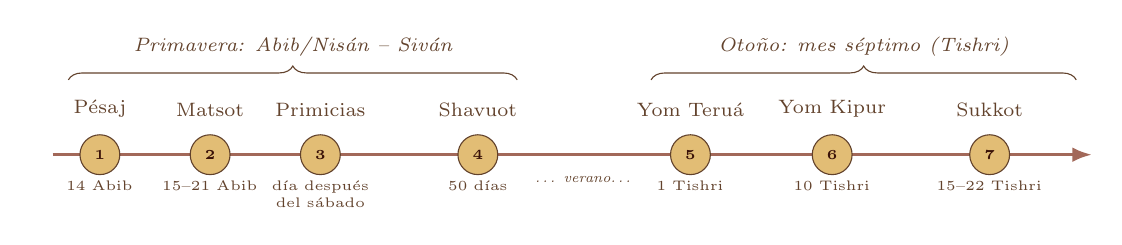
\begin{tikzpicture}[x=1cm,y=1cm,font=\scriptsize]
 \def\fiestaactual{0}
 \draw[line width=1.2pt,tierraroja!70,-{Latex[length=2.5mm]}] (0,0) -- (13.2,0);
 \draw[decorate,decoration={brace,amplitude=5pt},sepia] (0.2,0.95) -- (5.9,0.95) node[midway,above=5pt,font=\scriptsize\itshape]{Primavera: Abib/Nisán -- Siván};
 \draw[decorate,decoration={brace,amplitude=5pt},sepia] (7.6,0.95) -- (13.0,0.95) node[midway,above=5pt,font=\scriptsize\itshape]{Otoño: mes séptimo (Tishri)};
 \foreach \n/\x/\t/\d in {1/0.6/Pésaj/{14 Abib},2/2.0/Matsot/{15--21 Abib},3/3.4/Primicias/{día después del sábado},4/5.4/Shavuot/{50 días},5/8.1/Yom Teruá/{1 Tishri},6/9.9/Yom Kipur/{10 Tishri},7/11.9/Sukkot/{15--22 Tishri}}{
   \ifnum\n=\fiestaactual
     \node[circle,fill=tierraroja,draw=caferojizo,minimum size=5.5mm,text=papiro,font=\scriptsize\bfseries] at (\x,0) {\n};
     \node[above=3pt,font=\scriptsize\bfseries,text=tierraroja] at (\x,0.28) {\t};
   \else
     \node[circle,fill=mostaza!70,draw=sepia,minimum size=4.5mm,text=caferojizo,font=\tiny\bfseries] at (\x,0) {\n};
     \node[above=3pt,text=sepia] at (\x,0.25) {\t};
   \fi
   \node[below=6pt,text width=1.6cm,align=center,font=\tiny,text=sepia] at (\x,0) {\d};}
 \node[font=\tiny\itshape,text=sepia] at (6.75,-0.32) {\ldots\ verano\ldots};
\end{tikzpicture}\par
{\footnotesize\color{sepia}\textit{Figura 1.} El ciclo anual de Levítico 23. \textit{Nota.} Esquema estándar de la serie; en este estudio introductorio no se resalta ninguna fiesta. El Shabat semanal (Lv 23:3) atraviesa todo el ciclo.}
\end{center}

%===================================================================
\section{El texto: Levítico 23}\label{sec:texto}

\subsection{Los versículos de apertura}
El capítulo comienza con la fórmula que lo atraviesa de principio a fin y con un doble encabezado que rodea al Shabat:

\hebverso{וַיְדַבֵּר יְהוָה אֶל־מֹשֶׁה לֵּאמֹר \\ שֵׁשֶׁת יָמִים תֵּעָשֶׂה מְלָאכָה וּבַיּוֹם הַשְּׁבִיעִי שַׁבַּת שַׁבָּתוֹן מִקְרָא־קֹדֶשׁ \\ כָּל־מְלָאכָה לֹא תַעֲשׂוּ שַׁבָּת הִוא לַיהוָה בְּכֹל מוֹשְׁבֹתֵיכֶם \\ אֵלֶּה מוֹעֲדֵי יְהוָה מִקְרָאֵי קֹדֶשׁ אֲשֶׁר־תִּקְרְאוּ אֹתָם בְּמוֹעֲדָם}
\begin{cita}Habló \SENOR{} a Moisés, diciendo: [\ldots] Seis días se trabajará, mas el séptimo día será de reposo, santa convocación; ningún trabajo haréis; día de reposo es del \SENOR{} en dondequiera que habitéis. Estas son las fiestas solemnes del \SENOR, las convocaciones santas, a las cuales convocaréis en sus tiempos:\fuente{(Lv 23:1, 3--4)}\end{cita}

Tres rasgos merecen atención desde el comienzo. El sujeto es ``el \SENOR'': el capítulo presenta las fiestas como palabra divina y no como invención de Moisés ni costumbre del pueblo, y la fórmula vuelve cinco veces (vv. 1, 9, 23, 26, 33). El Shabat, por su parte, queda entre dos encabezados casi idénticos (vv. 2 y 4), como si el día séptimo fuera a la vez una de las citas y el fundamento de todas. Y las citas se proclaman \heb{בְּמוֹעֲדָם} (\emph{bemoadam}), ``en su tiempo señalado'': cada una tiene fecha, y la fecha la fija quien convoca.

\subsection{Recorrido del capítulo}
Levítico 23 avanza por el año desde el primer mes hasta el séptimo. Cada solemnidad recibe una fecha, una calificación (convocación santa, reposo, fiesta) y una prescripción sobre el trabajo y las ofrendas:

\begin{center}\small\renewcommand{\arraystretch}{1.18}
\begin{tabular}{@{}L{1.5cm}L{3.3cm}L{2.7cm}L{7.6cm}@{}}
\toprule
\textbf{Vv.} & \textbf{Solemnidad} & \textbf{Fecha} & \textbf{Prescripciones del texto} \\ \midrule
3 & Shabat & cada séptimo día & \emph{shabat shabatón}, convocación santa, ``ningún trabajo'' (\emph{kol melajá}), ``en dondequiera que habitéis'' \\
5 & Pascua (\emph{Pésaj}) & 14 del mes primero & ``entre las dos tardes''; no se llama convocación \\
6--8 & Panes sin levadura (\emph{Matsot}) & 15--21 del mes primero & \emph{jag}; siete días de ázimos; convocación el primero y el séptimo; ``ningún trabajo de siervos''; ofrenda encendida siete días \\
9--14 & Gavilla (\emph{ómer}) & ``el día siguiente del día de reposo'' & ``cuando hayáis entrado en la tierra''; primicia de la siega; holocausto, ofrenda, libación; no comer grano nuevo antes; ``estatuto perpetuo'' \\
15--21 & Semanas (\emph{Shavuot}) & 50 días contados & siete semanas; dos panes \emph{con} levadura; sacrificios; convocación; ``estatuto perpetuo'' \\
22 & (rebusco) & --- & no segar los rincones ni recoger lo caído: para el pobre y el extranjero \\
23--25 & Memorial de trompetas & 1 del mes séptimo & \emph{shabatón}, \emph{zijrón teruá}, convocación, ofrenda encendida \\
26--32 & Día de las expiaciones & 10 del mes séptimo & \emph{shabat shabatón}; ``afligiréis vuestras almas''; ``ningún trabajo''; ``de tarde a tarde'' \\
33--36 & Tabernáculos (\emph{Sukkot}) & 15--21 del mes séptimo & \emph{jag} de siete días; convocación el primero; ofrenda encendida siete días \\
36 & Octavo día (\emph{atséret}) & 22 del mes séptimo & convocación, ``es fiesta'' (\emph{atséret}), ``ningún trabajo de siervos'' \\
37--38 & Suscripción & --- & ``estas son las fiestas solemnes del \SENOR''; remite a las ofrendas de cada día \\
39--43 & Suplemento de Sukkot & 15--22 del mes séptimo & frutos, ramas de palmera y sauces; habitar en cabañas; ``para que sepan vuestros descendientes'' \\
44 & Cierre & --- & ``Así habló Moisés a los hijos de Israel sobre las fiestas solemnes del \SENOR'' \\
\bottomrule
\end{tabular}\par
{\footnotesize\color{sepia}\textit{Tabla 2.} Recorrido de Levítico 23. \textit{Nota.} Elaboración propia con la BHS y la RVR1960.}
\end{center}

La tabla deja ver que no todas las solemnidades son iguales, algo que una lectura rápida pasa por alto. La Pascua (v. 5) no recibe el título de convocación; es un sacrificio vespertino que abre la semana de ázimos. La gavilla del ómer tampoco es día de reposo, sino una ofrenda que inicia una cuenta. Los días de convocación santa con prohibición de trabajo son, por tanto, además del Shabat semanal, \destacar{siete al año}: el primero y el séptimo de Matsot, Shavuot, el primero del mes séptimo, el día diez, el primero de Sukkot y el octavo día. El siete que gobierna la semana gobierna también el año.

\subsection{Los textos del calendario en la Torá}
Levítico 23 no es el único calendario de la Torá. El Pentateuco contiene cinco textos festivos, cada uno con su aporte, y el calendario completo solo se obtiene leyéndolos juntos.

\begin{center}\small\renewcommand{\arraystretch}{1.18}
\begin{tabular}{@{}L{2.4cm}L{3.6cm}L{9.1cm}@{}}
\toprule
\textbf{Texto} & \textbf{Contexto} & \textbf{Lo que añade} \\ \midrule
Éx 23:14--17 & Código de la alianza & ``Tres veces en el año me celebraréis fiesta'' (\emph{shalosh regalim}): ázimos ``en el mes de Abib'', siega (\emph{katsir}), cosecha (\emph{asif}) ``a la salida del año''; nadie se presenta ``con las manos vacías'' \\
Éx 34:18--26 & Renovación del pacto tras el becerro & Los mismos tres tiempos; la fiesta de las semanas ``de las primicias de la siega del trigo''; la cosecha ``a la vuelta del año'' (trad. propia de \emph{tekufat hashaná}); primogénitos y Shabat ``aun en la arada y en la siega'' (34:21) \\
Lv 23 & Ley de santidad & El calendario completo con fechas exactas: Shabat, siete fiestas, convocaciones santas, prohibición de trabajo, suplemento de Sukkot \\
Nm 28--29 & Ofrendas públicas & Las ofrendas de cada tiempo: holocausto continuo, Shabat, lunas nuevas, cada fiesta; los setenta becerros de Sukkot \\
Dt 16:1--17 & Discurso de Moisés & ``El lugar que \SENOR{} escogiere''; Pascua ``de noche''; regocijo con el hijo, el siervo, el levita, el extranjero, el huérfano y la viuda \\
\bottomrule
\end{tabular}\par
{\footnotesize\color{sepia}\textit{Tabla 3.} Tabla sinóptica de los calendarios festivos de la Torá. \textit{Nota.} Elaboración propia con la RVR1960 y la BHS. Ez 45:18--25 ofrece además un calendario profético del templo futuro.}
\end{center}

Éxodo nombra las fiestas por la tierra (ázimos, siega, cosecha); Levítico, por el tiempo y la santidad (fecha, convocación, reposo); Números, por el altar (qué se ofrece); Deuteronomio, por el lugar y la comunidad (dónde y con quién se goza). La fiesta bíblica reúne todo eso: un tiempo fijado, una cosecha recogida, una ofrenda presentada, un viaje al santuario y una mesa compartida.

\subsection{Las tres peregrinaciones}
Tres de las fiestas son de peregrinación. Éxodo las llama \heb{שָׁלֹשׁ רְגָלִים} (\emph{shalosh regalim}), literalmente ``tres pies'', es decir, tres veces en que se va a pie:

\hebverso{שָׁלוֹשׁ פְּעָמִים בַּשָּׁנָה יֵרָאֶה כָל־זְכוּרְךָ אֶת־פְּנֵי יְהוָה אֱלֹהֶיךָ בַּמָּקוֹם אֲשֶׁר יִבְחָר \\ בְּחַג הַמַּצּוֹת וּבְחַג הַשָּׁבֻעוֹת וּבְחַג הַסֻּכּוֹת וְלֹא יֵרָאֶה אֶת־פְּנֵי יְהוָה רֵיקָם}
\begin{cita}Tres veces cada año aparecerá todo varón tuyo delante del \SENOR{} tu Dios en el lugar que él escogiere: en la fiesta solemne de los panes sin levadura, y en la fiesta solemne de las semanas, y en la fiesta solemne de los tabernáculos. Y ninguno se presentará delante del \SENOR{} con las manos vacías.\fuente{(Dt 16:16; cf. Éx 23:14--17; 34:23)}\end{cita}

Las tres comparten la palabra \heb{חַג} (\emph{jag}), la fiesta de peregrinación (§\ref{sec:filologia}). Las solemnidades del mes séptimo que no son \emph{jag} (el día de las trompetas y el de las expiaciones) no exigen viaje, y el Shabat tampoco, pues se guarda ``en dondequiera que habitéis''. Así queda trazada la geografía del calendario: el Shabat santifica la casa y las peregrinaciones llevan a la casa de Dios.

\begin{nota}[Precisión]
El verbo ``aparecerá'' (\heb{יֵרָאֶה}, \emph{yeraé}, nifal de \emph{raá}) es, según muchos comentaristas, una vocalización masorética que evita decir ``verá el rostro de Dios'' (qal \emph{yiré}); ``ver el rostro'' de un rey era fórmula de audiencia en el antiguo Cercano Oriente (Tigay, 1996). En cualquiera de las dos lecturas el peregrino va a presentarse ante su Señor, y no va con las manos vacías.
\end{nota}

%===================================================================
\section{Lectura histórica: cómo contaba Israel el tiempo}\label{sec:historia}

\subsection{Un calendario de luna y de sol}
El relato de la creación encarga a los astros algo más que alumbrar: ``Haya lumbreras en la expansión de los cielos para separar el día de la noche; y sirvan de señales para las estaciones, para días y años'' (Gn 1:14). La palabra traducida ``estaciones'' es \heb{וּלְמוֹעֲדִים} (\emph{ulemoadim}), la misma de Lv 23:2, de modo que el cielo ya está preparado para marcar las citas antes de que exista Israel. El Salmo lo repite: ``Hizo la luna para los tiempos'' (\heb{לְמוֹעֲדִים}; Sal 104:19).

El calendario de Israel es \destacar{lunisolar}. El mes comienza con la luna nueva; la palabra \heb{חֹדֶשׁ} (\emph{jódesh}) significa a la vez ``luna nueva'' y ``mes'' y viene de la raíz \emph{j-d-sh}, ``ser nuevo''. Doce lunaciones suman unos 354 días, once menos que el año solar, y las fiestas están atadas a cosechas que dependen del sol: la cebada madura en primavera y la uva en verano, haga lo que haga la luna. Un calendario puramente lunar haría retroceder la Pascua por todas las estaciones, como ocurre con los meses del calendario islámico. Israel necesitaba meses lunares y un año solar a la vez.

\subsection{La luna nueva y el Rosh Jódesh}
La luna nueva no figura en Levítico 23, pero era un tiempo sagrado. Números la incluye en el calendario de ofrendas (Nm 28:11--15) y en el toque de las trompetas de plata:

\hebverso{וּבְיוֹם שִׂמְחַתְכֶם וּבְמוֹעֲדֵיכֶם וּבְרָאשֵׁי חָדְשֵׁיכֶם \\ וּתְקַעְתֶּם בַּחֲצֹצְרֹת עַל עֹלֹתֵיכֶם}
\begin{cita}Y en el día de vuestra alegría, y en vuestras solemnidades, y en los principios de vuestros meses, tocaréis las trompetas sobre vuestros holocaustos, y sobre los sacrificios de paz, y os serán por memoria delante de vuestro Dios. Yo \SENOR{} vuestro Dios.\fuente{(Nm 10:10)}\end{cita}

Los relatos muestran que la luna nueva organizaba la vida. David sabe que ``mañana será nueva luna'' y que se espera su lugar en la mesa del rey (1~S 20:5, 18, 24--27); el marido de la sunamita le pregunta por qué va al profeta si ``no es nueva luna, ni día de reposo'' (2~R 4:23); los comerciantes de Amós preguntan ``¿Cuándo pasará el mes, y venderemos el trigo; y la semana, y abriremos los graneros del pan\ldots?'' (Am 8:5). El par ``luna nueva y sábado'' aparece en los profetas, a veces para condenar un culto vacío (Is 1:13--14; Os 2:11 [2:13]) y a veces como figura del culto final: ``de mes en mes, y de día de reposo en día de reposo, vendrán todos a adorar delante de mí, dijo \SENOR'' (Is 66:23; cf. Ez 46:1--3).

La fórmula ``fiestas, lunas nuevas y sábados'' resume el tiempo sagrado de Israel en sus tres ciclos, anual, mensual y semanal (1~Cr 23:31; 2~Cr 2:4 [2:3]; 8:13; 31:3; Ez 45:17; Os 2:11). Pablo la reproduce, en orden inverso, en Col 2:16: \grc{ἑορτῆς ἢ νουμηνίας ἢ σαββάτων}, ``días de fiesta, luna nueva o días de reposo''. Ese eco pesará en el debate de §\ref{sec:discusion}, porque muestra que Pablo habla del calendario de la Torá y no de un calendario pagano.

\subsection{Los nombres de los meses}
La Biblia nombra los meses de tres maneras, que corresponden a tres épocas:

\begin{center}\begin{minipage}{\linewidth}\centering\small\renewcommand{\arraystretch}{1.16}
\begin{tabular}{@{}L{0.6cm}L{2.2cm}L{2.0cm}L{1.6cm}L{3.8cm}L{4.1cm}@{}}
\toprule
\textbf{N.º} & \textbf{Nombre posexílico} & \textbf{Nombre antiguo} & \textbf{Aprox.} & \textbf{Campo y clima} & \textbf{Fiestas} \\ \midrule
1 & Nisán (Neh 2:1; Est 3:7) & Abib (Éx 13:4) & mar--abr & lluvia tardía; siega de la cebada & Pésaj, Matsot, ómer \\
2 & Iyar & Zif (1~R 6:1) & abr--may & siega de la cebada & (Pésaj segundo, Nm 9:11) \\
3 & Siván (Est 8:9) & --- & may--jun & siega del trigo & Shavuot \\
4 & Tamuz & --- & jun--jul & estación seca & --- \\
5 & Av & --- & jul--ago & uvas, higos & --- \\
6 & Elul (Neh 6:15) & --- & ago--sep & vendimia, fruta de verano & --- \\
7 & Tishri & Etanim (1~R 8:2) & sep--oct & recolección; primeras lluvias & Teruá, Kipur, Sukkot, octavo día \\
8 & Marjeshván & Bul (1~R 6:38) & oct--nov & lluvia temprana; aceituna; arado y siembra & --- \\
9 & Kislev (Zac 7:1) & --- & nov--dic & siembra & Janucá (Jn 10:22) \\
10 & Tevet (Est 2:16) & --- & dic--ene & lluvias de invierno & --- \\
11 & Shevat (Zac 1:7) & --- & ene--feb & lluvias de invierno & --- \\
12 & Adar (Esd 6:15; Est 3:7) & --- & feb--mar & lino; espigas & Purim (Est 9) \\
\bottomrule
\end{tabular}\par
{\footnotesize\color{sepia}\textit{Tabla 4.} Los meses del año hebreo. \textit{Nota.} Elaboración propia con la RVR1960 y de Vaux (1985). Iyar, Tamuz (como mes), Av, Tishri y Marjeshván no aparecen en la Biblia; se documentan en la literatura judía posterior. Las equivalencias gregorianas son aproximadas y se desplazan cada año.}
\end{minipage}\end{center}

La capa más antigua usa nombres cananeos, compartidos con los fenicios: \emph{Abib}, \emph{Zif}, \emph{Etanim} y \emph{Bul}. Aparecen en Éxodo, Deuteronomio y en el relato de la construcción del templo, que fecha sus etapas con ellos: ``en el mes de Zif, que es el mes segundo, comenzó él a edificar la casa del \SENOR'' (1~R 6:1); ``en el mes de Bul, que es el mes octavo'' se terminó (6:38); y la dedicación se hizo ``en el mes de Etanim, que es el mes séptimo'', en la fiesta (8:2). El narrador ya necesita explicar los nombres viejos con números, y esa segunda capa, la de los \destacar{ordinales} (``el mes primero'', ``el mes séptimo''), es la que usa la ley sacerdotal y la que domina Levítico 23. La tercera son los \destacar{nombres babilónicos} que los judíos trajeron del exilio: Nisán, Siván, Elul, Kislev, Tevet, Shevat y Adar aparecen en Ester, Nehemías y Zacarías, y ``el mes primero, que es el mes de Nisán'' (Est 3:7) muestra el empalme entre los sistemas. La Misná y el calendario judío actual siguen usando esta última.

\subsection{Abib, ``el principio de los meses''}
El nombre del primer mes es una descripción: \heb{אָבִיב} (\emph{aviv}) es la espiga ya formada, todavía verde. Cuando el granizo cae sobre Egipto, ``El lino, pues, y la cebada fueron destrozados, porque la cebada estaba ya espigada'' (\emph{haseorá aviv}, Éx 9:31). En el relato de la Pascua, Dios fija el comienzo del año:

\hebverso{הַחֹדֶשׁ הַזֶּה לָכֶם רֹאשׁ חֳדָשִׁים רִאשׁוֹן הוּא לָכֶם לְחָדְשֵׁי הַשָּׁנָה}
\begin{cita}Este mes os será principio de los meses; para vosotros será éste el primero en los meses del año.\fuente{(Éx 12:2)}\end{cita}

``Vosotros salís hoy en el mes de Abib'' (Éx 13:4); ``Guardarás el mes de Abib, y harás pascua al \SENOR{} tu Dios; porque en el mes de Abib te sacó el \SENOR{} tu Dios de Egipto, de noche'' (Dt 16:1; cf. Éx 23:15; 34:18). El año de Israel comienza, así, donde comenzó su libertad.

La Torá conoce también, sin embargo, un año que gira en otoño. La fiesta de la cosecha cae ``a la salida del año'' (\heb{בְּצֵאת הַשָּׁנָה}, Éx 23:16) o ``a la vuelta del año'' (\heb{תְּקוּפַת הַשָּׁנָה}, Éx 34:22), y el año de Jubileo se proclama el día diez del mes séptimo (Lv 25:9). Hay dos comienzos: uno litúrgico, en Abib, que cuenta los meses desde la Pascua, y otro agrícola, en otoño, que cierra un ciclo de cosechas y abre otro de siembra.

\begin{nota}[Precisión]
La Misná sistematiza cuatro ``años nuevos'': el 1 de Nisán para los reyes y las fiestas; el 1 de Elul para el diezmo del ganado; el 1 de Tishri para los años, la \emph{shemitá}, el Jubileo y las plantaciones; y el 1 (o el 15) de Shevat para los árboles (Misná, \emph{Rosh haShaná} 1:1). Llamar ``Rosh haShaná'' (año nuevo) al 1 de Tishri es uso rabínico: Lv 23:24 lo llama ``memorial de trompetas'' del mes séptimo. El estudio 05 de la serie lo examina.
\end{nota}

\subsection{El calendario de Gézer}
El testimonio extrabíblico más antiguo del año agrícola israelita es una pequeña tablilla de piedra caliza hallada en 1908 en Gézer por R. A. S. Macalister y conservada hoy en el Museo Arqueológico de Estambul. Se la fecha en el siglo X a.\,e.\,c., en la época de la monarquía unida. Sus siete líneas enumeran el año por labores:

\begin{cita}Dos meses de recolección (\emph{asif}); dos meses de siembra; dos meses de siembra tardía; un mes de corte del lino; un mes de siega de la cebada; un mes de siega y de medida; dos meses de poda (o vendimia); un mes de fruta de verano (\emph{kayits}).\fuente{(Calendario de Gézer, trad. propia)}\end{cita}

Los meses suman doce, y la lista empieza con el \emph{asif}, la recolección otoñal, el mismo término que Éx 23:16 da a la fiesta que cae ``a la salida del año''. La tablilla no menciona fiestas, pero muestra la tierra en que se celebraban: la cebada de la Pascua y del ómer, el trigo de Shavuot, la fruta y la vendimia que preceden a Sukkot.

\begin{nota}[Precisión]
La lectura de algunos términos de Gézer es discutida: \emph{zamir} puede ser ``poda'' o ``vendimia'', y la palabra que acompaña a la siega del trigo puede leerse ``y medida'' o ``y fiesta''. Tampoco hay acuerdo sobre si la escritura es paleohebrea o fenicia, ni sobre la función del texto (ejercicio escolar, canción mnemotécnica o registro). Lo seguro es su orden agrícola y su comienzo en otoño (de Vaux, 1985).
\end{nota}

\subsection{Lluvias y cosechas}
A diferencia de Egipto, que riega con su río, la tierra de Israel ``bebe las aguas de la lluvia del cielo'' (Dt 11:11). Su año tiene dos estaciones, una lluviosa, de octubre a abril, y una seca, de mayo a septiembre. La lluvia que abre la estación se llama \heb{יוֹרֶה} (\emph{yoré}), ``temprana'', y ablanda la tierra para el arado; la que la cierra, \heb{מַלְקוֹשׁ} (\emph{malkosh}), ``tardía'', llena las espigas antes de la siega:

\begin{cita}Yo daré la lluvia de vuestra tierra a su tiempo, la temprana y la tardía; y recogerás tu grano, tu vino y tu aceite.\fuente{(Dt 11:14; cf. Jer 5:24; Jl 2:23; Stg 5:7)}\end{cita}

Las fiestas siguen el calendario de las cosechas. La cebada madura primero, en Abib: Rut llega a Belén ``al comienzo de la siega de la cebada'' (Rt 1:22), y la gavilla del ómer la ofrece al \SENOR{} antes de que nadie la coma (Lv 23:14). Siete semanas después madura el trigo, y Shavuot es ``la fiesta de las semanas, la de las primicias de la siega del trigo'' (Éx 34:22); Rut espiga ``hasta que se acabó la siega de la cebada y la del trigo'' (Rt 2:23). En verano se cosechan higos y uvas; a fines del verano, la vendimia y el comienzo de la aceituna. Sukkot, la fiesta de la cosecha, llega cuando ``hayáis recogido el fruto de la tierra'' (Lv 23:39), justo antes de que caiga la lluvia temprana. Por eso la tradición judía introduce en el octavo día la oración por la lluvia, y por eso Zacarías amenaza con sequía a las naciones que no suban a la fiesta (Zac 14:17).

Los profetas tomaron las dos cosechas como imágenes del juicio final. La siega del grano y la vendimia que precede a Sukkot vuelven en el oráculo de Joel: ``Echad la hoz, porque la mies está ya madura. Venid, descended, porque el lagar está lleno'' (Jl 3:13 [4:13]); en Isaías, el que viene de Edom ``con vestidos rojos'' ha pisado solo el lagar (Is 63:1--6; cf. 24:1--13; 32:9--13); y en el Apocalipsis un ángel siega ``la mies de la tierra'' y otro vendimia ``los racimos'' para ``el gran lagar de la ira de Dios'' (Ap 14:14--20; cf. 19:15). En mis presentaciones anteriores he insistido en esta lectura: el ciclo agrícola de las fiestas es también un calendario del fin.

\subsection{La intercalación: un mes de más}
Si el año de doce lunas es once días más corto que el solar, cada dos o tres años la Pascua quedaría antes de la espiga. La Torá no legisla un mes adicional, pero su exigencia de celebrar la Pascua ``en el mes de Abib'', el mes de la espiga, obliga a ajustar el calendario. La práctica judía documentada es añadir un decimotercer mes, \emph{Adar sheni} (Adar segundo, también llamado \emph{Veadar}), antes de Nisán.

\begin{nota}[Precisión]
La intercalación es práctica rabínica atestiguada en la Misná y el Talmud: el tribunal decidía añadir el mes según el estado de la cebada, los frutos y la \emph{tekufá} solar (Tosefta, \emph{Sanedrín} 2:2; Talmud Babilónico, \emph{Sanedrín} 11b), y la luna nueva se proclamaba por testigos (Misná, \emph{Rosh haShaná} 1--2). El calendario fijo actual, con siete años bisiestos en cada ciclo de diecinueve, se atribuye por tradición a Hilel~II (siglo IV e.\,c.); la noticia procede de fuentes medievales. Los caraítas, en cambio, siguen observando la espiga de cebada (\emph{aviv}) para fijar el año. La Biblia no describe ningún método de intercalación.
\end{nota}

\subsection{Otro calendario: los 364 días de Jubileos y Qumrán}
En el siglo II a.\,e.\,c. circulaba en Judea un calendario rival, solar y esquemático, de 364 días: exactamente 52 semanas, cuatro trimestres de 91 días. Lo defienden el \emph{Libro astronómico} de 1 Enoc (caps. 72--82) y el libro de los Jubileos, que acusa a quienes siguen la luna de ``confundir'' las fiestas (Jub 6:32--38), y lo usan los manuscritos de Qumrán, entre ellos los turnos sacerdotales de 4Q320--330 y el calendario festivo del \emph{Rollo del Templo} (VanderKam, 1998). En ese sistema el año empieza en miércoles, el día en que fueron creadas las lumbreras, y cada fiesta cae siempre en el mismo día de la semana. El \emph{Documento de Damasco} considera que Israel se extravió precisamente en ``sus sábados santos y sus fiestas gloriosas'' (CD 3:14--15; García Martínez, 1992).

La disputa muestra que en tiempos de Jesús el calendario era una cuestión teológica antes que técnica: guardar la cita de Dios en el día equivocado era faltar a la cita.

\subsection{Línea de tiempo y rueda del año}
La figura 2 ordena los testimonios del calendario que acabo de recorrer; la figura 3 reúne en una rueda los meses, las estaciones, las cosechas y las fiestas.

\begin{center}
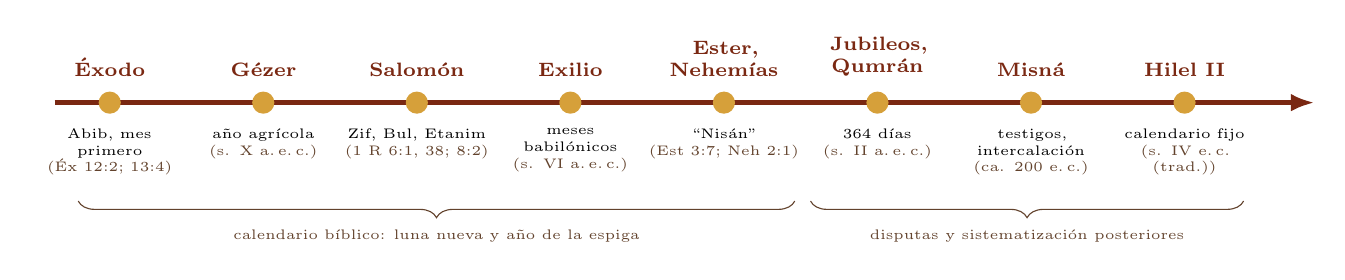
\begin{tikzpicture}[font=\scriptsize]
 \draw[line width=1.6pt,tierraroja,-{Latex[length=3mm]}] (0,0) -- (16.0,0);
 \foreach \x/\a/\b/\c in {0.7/{Éxodo}/{Abib, mes primero}/{Éx 12:2; 13:4}, 2.65/{Gézer}/{año agrícola}/{s. X a.\,e.\,c.}, 4.6/{Salomón}/{Zif, Bul, Etanim}/{1 R 6:1, 38; 8:2}, 6.55/{Exilio}/{meses babilónicos}/{s. VI a.\,e.\,c.}, 8.5/{Ester, Nehemías}/{``Nisán''}/{Est 3:7; Neh 2:1}, 10.45/{Jubileos, Qumrán}/{364 días}/{s. II a.\,e.\,c.}, 12.4/{Misná}/{testigos, intercalación}/{ca. 200 e.\,c.}, 14.35/{Hilel II}/{calendario fijo}/{s. IV e.\,c. (trad.)}}{
   \fill[mostaza] (\x,0) circle (4pt);
   \node[above=6pt,font=\scriptsize\bfseries,text=tierraroja,text width=1.85cm,align=center] at (\x,0) {\a};
   \node[below=6pt,text width=1.85cm,align=center,font=\tiny] at (\x,0) {\b\\ \textcolor{sepia}{(\c)}};}
 \draw[decorate,decoration={brace,amplitude=6pt,mirror},sepia] (0.3,-1.25) -- (9.4,-1.25) node[midway,below=7pt,font=\tiny,text=sepia] {calendario bíblico: luna nueva y año de la espiga};
 \draw[decorate,decoration={brace,amplitude=6pt,mirror},sepia] (9.6,-1.25) -- (15.1,-1.25) node[midway,below=7pt,font=\tiny,text=sepia] {disputas y sistematización posteriores};
\end{tikzpicture}\par
{\footnotesize\color{sepia}\textit{Figura 2.} Testimonios del calendario de Israel. \textit{Nota.} Elaboración propia. La fecha del éxodo es discutida (véase §\ref{sec:serie}).}
\end{center}

\begin{center}
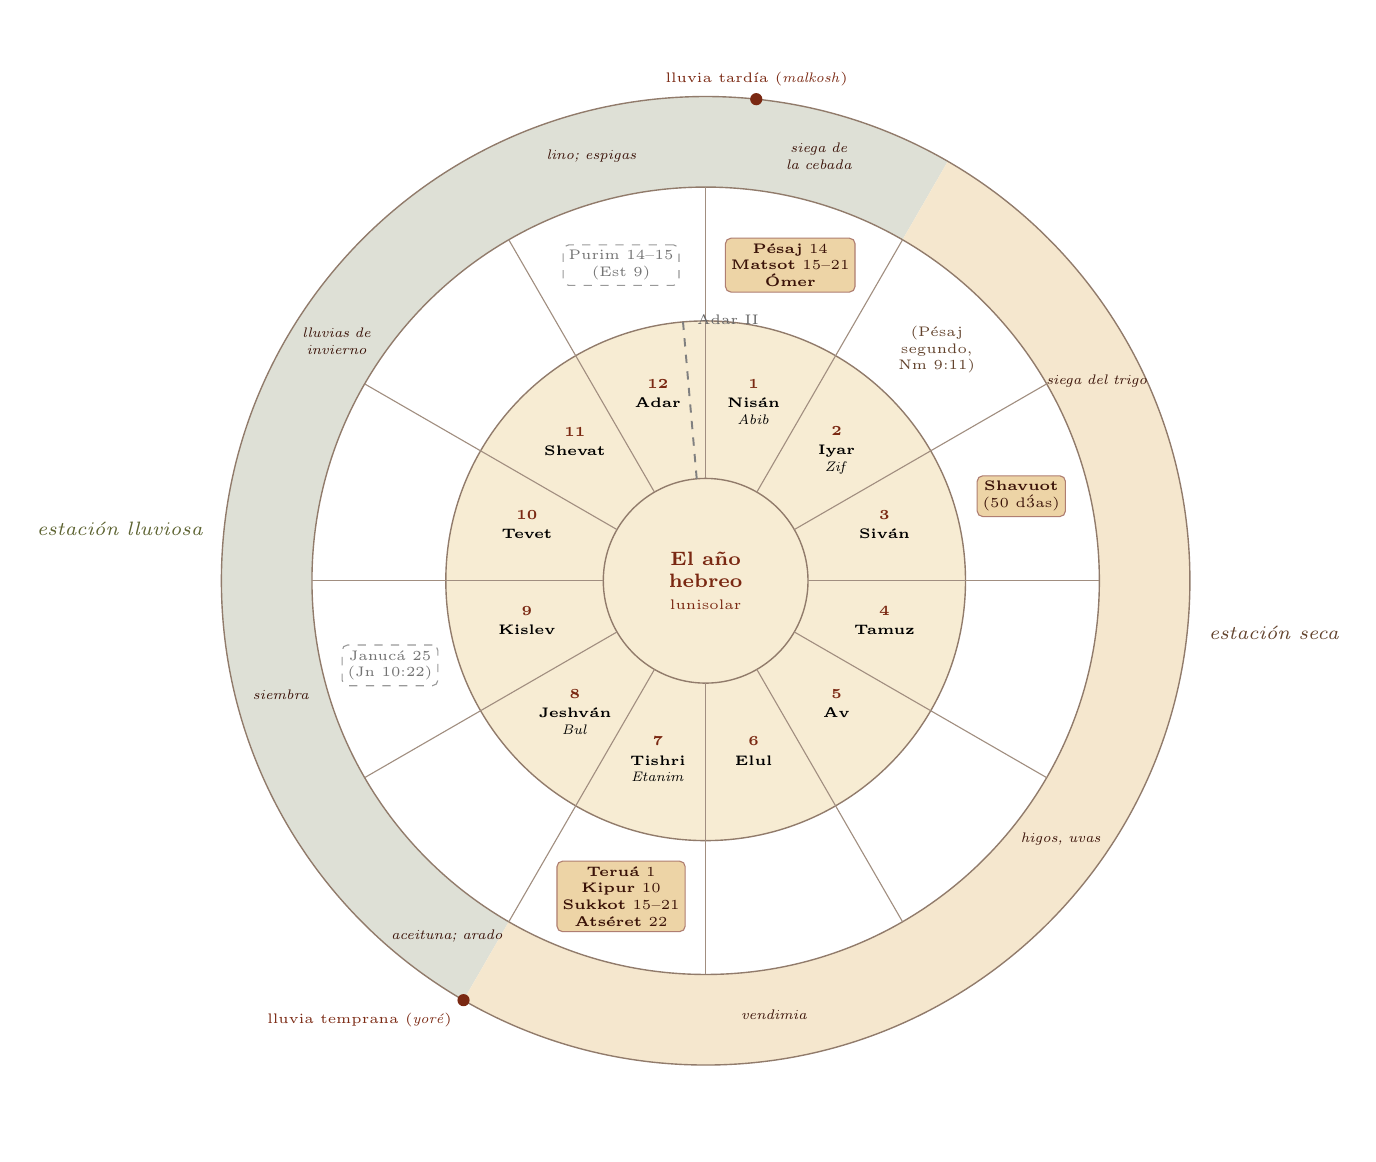
\begin{tikzpicture}[font=\scriptsize]
 % estaciones (anillo exterior): lluviosa = meses 8 a 1; seca = meses 2 a 7 (arriba = inicio de Nisán; sentido horario)
 \fill[oliva!20] (0,0) -- ({90-7*30}:6.15) arc[start angle={90-7*30},end angle={90-13*30},radius=6.15] -- cycle;
 \fill[mostaza!25] (0,0) -- ({90-1*30}:6.15) arc[start angle={90-1*30},end angle={90-7*30},radius=6.15] -- cycle;
 \fill[white] (0,0) circle (5.0);
 \fill[papiro!70] (0,0) circle (3.3);
 \draw[sepia!70,line width=0.5pt] (0,0) circle (1.3) circle (3.3) circle (5.0) circle (6.15);
 \foreach \i in {0,...,11}{\draw[sepia!60,line width=0.4pt] ({90-\i*30}:1.3) -- ({90-\i*30}:5.0);}
 \foreach \i/\n/\o in {1/Nisán/Abib,2/Iyar/Zif,3/Siván/{},4/Tamuz/{},5/Av/{},6/Elul/{},7/Tishri/Etanim,8/Jeshván/Bul,9/Kislev/{},10/Tevet/{},11/Shevat/{},12/Adar/{}}{
   \node[align=center,inner sep=0pt,font=\tiny] at ({90-(\i-0.5)*30}:2.35) {\textbf{\textcolor{tierraroja}{\i}}\\[1pt] \textbf{\n}\\ \textit{\o}};}
 \foreach \i/\t in {1/{\textbf{Pésaj} 14\\ \textbf{Matsot} 15--21\\ \textbf{Ómer}}, 3/{\textbf{Shavuot}\\ (50 días)}, 7/{\textbf{Teruá} 1\\ \textbf{Kipur} 10\\ \textbf{Sukkot} 15--21\\ \textbf{Atséret} 22}}{
   \node[align=center,font=\tiny,text=caferojizo,fill=mostaza!45,draw=tierraroja!60,rounded corners=2pt,inner sep=2pt] at ({90-(\i-0.5)*30}:4.15) {\t};}
 \node[align=center,font=\tiny,text=sepia] at ({90-(2-0.5)*30}:4.15) {(Pésaj\\ segundo,\\ Nm 9:11)};
 \node[align=center,font=\tiny,text=black!55,draw=black!40,dashed,rounded corners=2pt,inner sep=2pt] at ({90-(9-0.5)*30}:4.15) {Janucá 25\\ (Jn 10:22)};
 \node[align=center,font=\tiny,text=black!55,draw=black!40,dashed,rounded corners=2pt,inner sep=2pt] at ({90-(12-0.5)*30}:4.15) {Purim 14--15\\ (Est 9)};
 \draw[black!50,dashed,line width=0.7pt] ({90-12*30+5}:1.3) -- ({90-12*30+5}:3.3);
 \node[font=\tiny,text=black!60,anchor=west] at ({90-12*30+4}:3.33) {Adar II};
 \foreach \i/\t in {1.0/{siega de la cebada}, 2.6/{siega del trigo}, 4.7/{higos, uvas}, 6.2/{vendimia}, 7.7/{aceituna; arado}, 9.0/{siembra}, 10.6/{lluvias de invierno}, 12.0/{lino; espigas}}{
   \node[font=\tiny\itshape,text=caferojizo,align=center,text width=1.4cm] at ({90-(\i-0.5)*30}:5.58) {\t};}
 \fill[tierraroja] ({90-7*30}:6.15) circle (2.2pt); \node[font=\tiny,text=tierraroja,anchor=north east] at ({90-7*30}:6.2) {lluvia temprana (\emph{yoré})};
 \fill[tierraroja] ({90-0.2*30}:6.15) circle (2.2pt); \node[font=\tiny,text=tierraroja,anchor=south] at ({90-0.2*30}:6.2) {lluvia tardía (\emph{malkosh})};
 \node[font=\scriptsize\itshape,text=sepia,anchor=west] at ({90-3.2*30}:6.3) {estación seca};
 \node[font=\scriptsize\itshape,text=oliva,anchor=east] at ({90-9.2*30}:6.3) {estación lluviosa};
 \node[align=center,font=\scriptsize,text=tierraroja] at (0,0) {\textbf{El año}\\ \textbf{hebreo}\\ \tiny lunisolar};
\end{tikzpicture}\par
{\footnotesize\color{sepia}\textit{Figura 3.} La rueda del año hebreo. \textit{Nota.} Elaboración propia, a partir del ciclo de mis presentaciones anteriores. Meses posexílicos en negrita y antiguos en cursiva; el año comienza arriba y avanza en sentido horario. Fiestas de Levítico 23 en recuadros mostaza; Janucá y Purim, fiestas no levíticas, en gris discontinuo. Adar II (Veadar) es el mes intercalar de la práctica rabínica.}
\end{center}

%===================================================================
\section{El Shabat: la primera de las solemnidades}\label{sec:shabat}

Levítico 23 pone el Shabat antes que cualquier fiesta anual, y hay razones para ese orden: el día séptimo es la cita más frecuente, la más antigua en el relato bíblico y la raíz de los ciclos de siete que el capítulo despliega. Sigamos su recorrido por la Escritura, desde la creación hasta Hebreos, para llegar después a la lectura de la serie y a los debates.

\subsection{El séptimo día de la creación (Gn 2:1--3)}

\hebverso{וַיְכַל אֱלֹהִים בַּיּוֹם הַשְּׁבִיעִי מְלַאכְתּוֹ אֲשֶׁר עָשָׂה וַיִּשְׁבֹּת בַּיּוֹם הַשְּׁבִיעִי מִכָּל־מְלַאכְתּוֹ אֲשֶׁר עָשָׂה \\ וַיְבָרֶךְ אֱלֹהִים אֶת־יוֹם הַשְּׁבִיעִי וַיְקַדֵּשׁ אֹתוֹ כִּי בוֹ שָׁבַת מִכָּל־מְלַאכְתּוֹ אֲשֶׁר־בָּרָא אֱלֹהִים לַעֲשׂוֹת}
\begin{cita}Y acabó Dios en el día séptimo la obra que hizo; y reposó el día séptimo de toda la obra que hizo. Y bendijo Dios al día séptimo, y lo santificó, porque en él reposó de toda la obra que había hecho en la creación.\fuente{(Gn 2:2--3)}\end{cita}

\begin{filologia}[Gn 2:2--3]
\begin{tabular}{@{}L{3.1cm}L{1.5cm}L{10.2cm}@{}}
\heb{וַיִּשְׁבֹּת} \emph{vayishbot} & \heb{שׁבת} & ``y cesó''. La RVR1960 traduce ``reposó''. El verbo \emph{shavat} significa primero ``cesar, detenerse'': el maná ``cesó'' cuando Israel comió del fruto de Canaán (Jos 5:12). El reposo de Dios no es cansancio, es obra terminada. \\[2pt]
\heb{וַיְבָרֶךְ} \emph{vayevárej} & \heb{ברך} & ``y bendijo'': Dios bendijo a los animales (1:22) y al ser humano (1:28); ahora bendice un \emph{tiempo}. \\[2pt]
\heb{וַיְקַדֵּשׁ} \emph{vaykadesh} & \heb{קדשׁ} & ``y lo santificó'': primera vez que aparece la raíz \emph{k-d-sh} en la Biblia. Lo primero que Dios declara santo no es un lugar ni una persona, sino un día. \\[2pt]
\heb{מְלַאכְתּוֹ} \emph{melajtó} & \heb{מלאך} & ``su obra'' (\emph{melajá}): la misma palabra de la prohibición ``ningún trabajo (\emph{kol melajá}) haréis'' (Lv 23:3). El Shabat humano imita el cese divino. \\
\end{tabular}
\end{filologia}

La forma del pasaje acompaña a su contenido. ``El día séptimo'' se repite tres veces, y cada una de las tres oraciones que lo contienen tiene siete palabras hebreas: \emph{vaychal Elohim bayom hashevií melajtó asher asá}; \emph{vayishbot bayom hashevií mikol melajtó asher asá}; \emph{vayevárej Elohim et yom hashevií vaykadesh otó}. El párrafo completo (Gn 2:1--3) suma 35 palabras, cinco veces siete, como Gn 1:1 suma siete (Wenham, 1987; conteo propio sobre el Códice de Leningrado: 5 + 14 + 16 palabras en los vv. 1, 2 y 3). El día séptimo es, además, el único que no se cierra con ``y fue la tarde y la mañana''.

\begin{nota}[Precisión]
Los conteos son propios, sobre el Códice de Leningrado (base de la BHS), contando como palabras separadas las unidas por \emph{makaf}. La ausencia de la fórmula ``tarde y mañana'' en el día séptimo es un dato del texto; su lectura como ``día sin fin'' es interpretación antigua (Agustín, \emph{Confesiones} XIII) y no está explícita. Génesis 2 tampoco usa el sustantivo \emph{shabat} ni da un mandato a Adán: si el día séptimo es desde la creación una ordenanza para la humanidad o se convierte en mandamiento en el Sinaí es un debate abierto. Bacchiocchi (1977) defiende lo primero; A. T. Lincoln, en el volumen editado por Carson (1982), lo segundo.
\end{nota}

\subsection{El maná: el Shabat antes del Sinaí (Éx 16)}
El sustantivo \emph{shabat} aparece por primera vez en el desierto de Sin, antes de la entrega de la Ley. El maná cae seis días; el sexto, doble porción; el séptimo, nada:

\hebverso{שַׁבָּתוֹן שַׁבַּת־קֹדֶשׁ לַיהוָה מָחָר}
\begin{cita}Mañana es el santo día de reposo, el reposo consagrado al \SENOR{}\ldots{} Mirad que el \SENOR{} os dio el día de reposo, y por eso en el sexto día os da pan para dos días.\fuente{(Éx 16:23, 29)}\end{cita}

Antes de ser ley escrita en piedra, el Shabat es un ritmo impreso en el pan de cada día: Dios provee seis días y garantiza el séptimo, y el pueblo lo aprende comiendo. El Shabat se conoce, pues, antes del Sinaí; Gn 26:5 dice además que Abraham ``guardó mi precepto, mis mandamientos, mis estatutos y mis leyes''.

\subsection{Acuérdate y guarda: Éx 20 y Dt 5}
El cuarto mandamiento aparece dos veces en la Torá, con dos verbos y dos motivos:

\begin{center}\small\renewcommand{\arraystretch}{1.2}
\begin{tabular}{@{}L{2.4cm}L{6.2cm}L{6.6cm}@{}}
\toprule
 & \textbf{Éx 20:8--11} & \textbf{Dt 5:12--15} \\ \midrule
Verbo & \heb{זָכוֹר} \emph{zajor}, ``Acuérdate del día de reposo'' & \heb{שָׁמוֹר} \emph{shamor}, ``Guardarás el día de reposo'' \\
Beneficiarios & tú, hijo, hija, siervo, criada, bestia, extranjero & añade ``tu buey, ni tu asno'' y ``para que descanse tu siervo y tu sierva como tú'' \\
Motivo & ``Porque en seis días hizo el \SENOR{} los cielos y la tierra\ldots{} y reposó en el séptimo día'' (creación) & ``Acuérdate que fuiste siervo en tierra de Egipto, y que el \SENOR{} tu Dios te sacó de allá'' (liberación) \\
Verbo final & ``el \SENOR{} bendijo el día de reposo y lo santificó'' & ``te ha mandado que guardes el día de reposo'' \\
\bottomrule
\end{tabular}\par
{\footnotesize\color{sepia}\textit{Tabla 5.} El mandamiento del Shabat en sus dos versiones. \textit{Nota.} Elaboración propia con la BHS y la RVR1960.}
\end{center}

Las dos versiones se completan. Éxodo funda el Shabat en el orden de la creación: el ser humano descansa porque Dios descansó. Deuteronomio lo funda en la redención: el israelita descansa, y deja descansar a su siervo, porque él mismo fue esclavo y Dios lo liberó. El Shabat recuerda a la vez quién hizo el mundo y quién rompió las cadenas, y esa doble raíz anticipa la doble función de todas las fiestas, memorial de la obra de Dios y señal de su pueblo.

\begin{center}
\begin{tikzpicture}[font=\small]
 \node[draw=tierraroja,line width=0.8pt,fill=papiro,rounded corners=3pt,text width=4.6cm,align=center,inner sep=6pt] (ex) at (-4.6,0) {\textbf{\textcolor{tierraroja}{Éx 20:8--11}}\\ \heb{זָכוֹר} \emph{zajor}, ``acuérdate''\\[2pt] \footnotesize Dios creó en seis días y reposó\\ \textit{memorial de la creación}\\ (Gn 2:2--3)};
 \node[draw=tierraroja,line width=0.8pt,fill=papiro,rounded corners=3pt,text width=4.6cm,align=center,inner sep=6pt] (dt) at (4.6,0) {\textbf{\textcolor{tierraroja}{Dt 5:12--15}}\\ \heb{שָׁמוֹר} \emph{shamor}, ``guarda''\\[2pt] \footnotesize Dios sacó a Israel de Egipto\\ \textit{memorial de la liberación}\\ (Éx 12--14)};
 \node[draw=mostaza,line width=1.6pt,fill=tierraroja,text=papiro,rounded corners=3pt,text width=3.4cm,align=center,inner sep=6pt] (sh) at (0,-2.6) {\textbf{Shabat}\\ \heb{שַׁבָּת לַיהוָה}\\ \footnotesize ``señal'' (Éx 31:13, 17)};
 \draw[-{Latex[length=3mm]},mostaza,line width=1.4pt] (ex.south) to[out=-90,in=180] (sh.west);
 \draw[-{Latex[length=3mm]},mostaza,line width=1.4pt] (dt.south) to[out=-90,in=0] (sh.east);
 \node[font=\footnotesize\itshape,text=sepia,align=center] at (0,0) {el Creador\\ y el Redentor};
\end{tikzpicture}\par
{\footnotesize\color{sepia}\textit{Figura 4.} Las dos raíces del Shabat. \textit{Nota.} Elaboración propia.}
\end{center}

\begin{nota}[Precisión]
La tradición judía armoniza las dos versiones diciendo que \emph{zajor} y \emph{shamor} ``fueron dichos en una sola palabra'' (Mejiltá a Éx 20:8; Talmud Babilónico, \emph{Shevuot} 20b), fórmula que el himno \emph{Lejá dodí} (siglo XVI) canta cada viernes; es una lectura rabínica. La crítica histórica explica la diferencia por la diversa composición de Éxodo y Deuteronomio; para el lector canónico, las dos motivaciones conviven en el mismo Sinaí (Tigay, 1996).
\end{nota}

\subsection{Una señal y un pacto perpetuo (Éx 31:12--17)}
Al terminar las instrucciones del tabernáculo, Dios vuelve al Shabat:

\hebverso{וְשָׁמְרוּ בְנֵי־יִשְׂרָאֵל אֶת־הַשַּׁבָּת לַעֲשׂוֹת אֶת־הַשַּׁבָּת לְדֹרֹתָם בְּרִית עוֹלָם \\ בֵּינִי וּבֵין בְּנֵי יִשְׂרָאֵל אוֹת הִוא לְעֹלָם \foreignlanguage{spanish}{[\ldots]} וּבַיּוֹם הַשְּׁבִיעִי שָׁבַת וַיִּנָּפַשׁ}
\begin{cita}Guardarán, pues, el día de reposo los hijos de Israel, celebrándolo por sus generaciones por pacto perpetuo. Señal es para siempre entre mí y los hijos de Israel; porque en seis días hizo el \SENOR{} los cielos y la tierra, y en el séptimo día cesó y reposó.\fuente{(Éx 31:16--17; cf. 31:13; Ez 20:12, 20)}\end{cita}

El pasaje define el Shabat con cuatro rasgos. Es \heb{אוֹת} (\emph{ot}), ``señal'', como el arco iris del pacto con Noé (Gn 9:12--13) y la circuncisión del pacto con Abraham (Gn 17:11). Es \heb{בְּרִית עוֹלָם} (\emph{berit olam}), ``pacto perpetuo''. Tiene un propósito pedagógico, ``para que sepáis que yo soy el \SENOR{} que os santifico'' (31:13). Y descansa en el relato de la creación con un verbo poco esperado, \heb{וַיִּנָּפַשׁ} (\emph{vayinafash}), ``y tomó aliento'', derivado de \emph{néfesh}: Dios ``respiró''. El contexto añade la gravedad del mandato (31:14--15) y su lugar en el libro: el tabernáculo, espacio santo, se construye en seis días de trabajo y se detiene ante el tiempo santo. De esa vecindad deriva la tradición rabínica las 39 clases de trabajo prohibidas en Shabat (Misná, \emph{Shabat} 7:2; Talmud Babilónico, \emph{Shabat} 49b).

\subsection{En Levítico 23: ``en dondequiera que habitéis''}
Levítico 23:3 suma al Shabat los títulos de las fiestas: es \heb{שַׁבַּת שַׁבָּתוֹן} (\emph{shabat shabatón}), ``reposo solemne'', y \emph{mikrá kódesh}, convocación santa. Dos detalles lo distinguen de las fiestas anuales. La prohibición es total, ``ningún trabajo haréis'' (\emph{kol melajá lo taasú}), igual que en el día de las expiaciones (vv. 28, 31), mientras que en los demás días santos se prohíbe solo ``trabajo de siervos'' (\emph{melejet avodá}; vv. 7, 8, 21, 25, 35, 36). Y el lugar es ``en dondequiera que habitéis'' (\emph{bejol moshvoteijem}): el Shabat no exige peregrinar, se guarda en cada casa y en cada aldea, y por eso pudo sobrevivir al exilio cuando no había templo.

\subsection{Los profetas: delicia, frontera y señal para las naciones}
Para los profetas el Shabat es mucho más que un detalle ritual. Isaías lo abre a los extranjeros y a los eunucos, excluidos de la asamblea por otras leyes (Dt 23:1--3):

\hebverso{וּבְנֵי הַנֵּכָר הַנִּלְוִים עַל־יְהוָה \foreignlanguage{spanish}{[\ldots]} כָּל־שֹׁמֵר שַׁבָּת מֵחַלְּלוֹ וּמַחֲזִיקִים בִּבְרִיתִי}
\begin{cita}Y a los hijos de los extranjeros que sigan al \SENOR{} para servirle, y que amen el nombre del \SENOR{} para ser sus siervos; a todos los que guarden el día de reposo para no profanarlo, y abracen mi pacto, yo los llevaré a mi santo monte, y los recrearé en mi casa de oración\ldots{} porque mi casa será llamada casa de oración para todos los pueblos.\fuente{(Is 56:6--7)}\end{cita}

Jesús citará el final de este oráculo al purificar el templo (Mc 11:17). Dos capítulos después, Isaías define el Shabat por su espíritu: ``Si retrajeres del día de reposo tu pie, de hacer tu voluntad en mi día santo, y lo llamares delicia (\heb{עֹנֶג}, \emph{óneg}), santo, glorioso del \SENOR\ldots{} entonces te deleitarás en el \SENOR'' (Is 58:13--14). Jeremías lo convierte en frontera de la ciudad: ``Guardaos por vuestra vida de llevar carga en el día de reposo, y de meterla por las puertas de Jerusalén'' (Jer 17:21; cf. 17:19--27). Ezequiel lo llama señal (Ez 20:12, 20) y denuncia su profanación (20:13; 22:8, 26). Después del exilio, Nehemías cierra las puertas de Jerusalén ``cuando iba oscureciendo\ldots{} antes del día de reposo'' para impedir el comercio de los tirios (Neh 13:15--22; cf. 10:31). Para entonces el Shabat se ha vuelto marca de identidad de un pueblo disperso.

\subsection{Jesús y el día de reposo}
Los evangelios presentan a Jesús en la sinagoga ``en el día de reposo\ldots{} conforme a su costumbre'' (Lc 4:16). Sus conflictos con los fariseos versan sobre cómo guardar el Shabat, no sobre si guardarlo: si es lícito arrancar espigas por hambre (Mc 2:23--26), sanar (Mc 3:1--6; Lc 13:10--17; 14:1--6; Jn 5:1--18; 9:14) o hacer el bien. La respuesta de Jesús tiene dos partes:

\begin{cita}También les dijo: El día de reposo fue hecho por causa del hombre, y no el hombre por causa del día de reposo. Por tanto, el Hijo del Hombre es Señor aun del día de reposo.\fuente{(Mc 2:27--28)}\end{cita}

La primera parte recoge Éx 16:29 (``el \SENOR{} os dio el día de reposo'') y Dt 5:15: el Shabat es don. La segunda reclama autoridad sobre el don. En Lc 13, Jesús sana a una mujer encorvada dieciocho años y razona desde la lógica de Dt 5: ``a esta hija de Abraham, que Satanás había atado dieciocho años, ¿no se le debía desatar de esta ligadura en el día de reposo?'' (13:16). Si el Shabat recuerda la liberación de Egipto, ningún día es más apto para desatar. En Juan la defensa es teológica: ``Mi Padre hasta ahora trabaja, y yo trabajo'' (Jn 5:17).

Tras la crucifixión, Lucas anota que las mujeres ``descansaron el día de reposo, conforme al mandamiento'' (Lc 23:56). El dato se refiere a los discípulos más cercanos, en las horas entre la cruz y la resurrección; cuánto pesa ese dato frente a otros (Hch 20:7; 1~Co 16:2; Ap 1:10) forma parte del debate que expongo al final de esta sección.

\subsection{``Queda un reposo para el pueblo de Dios'' (He 3:7--4:11)}
La carta a los Hebreos lee el Shabat junto con el Salmo 95: ``juré en mi furor que no entrarían en mi reposo'' (Sal 95:11; He 3:11). La generación del desierto no entró en la tierra por incredulidad; Josué introdujo a la siguiente, pero el Salmo, escrito siglos después, todavía invita: ``Si oyereis hoy su voz''. De ahí nace el argumento:

\begin{cita}Porque si Josué les hubiera dado el reposo, no hablaría después de otro día. Por tanto, queda un reposo para el pueblo de Dios. Porque el que ha entrado en su reposo, también ha reposado de sus obras, como Dios de las suyas.\fuente{(He 4:8--10)}\end{cita}

\begin{filologia}[He 4:9]
\begin{tabular}{@{}L{3.4cm}L{2.1cm}L{9.3cm}@{}}
\grc{κατάπαυσις} \emph{katápausis} & Sal 95:11 LXX & ``reposo'', ``lugar de descanso'': la palabra de la LXX para \heb{מְנוּחָה} (\emph{menujá}), el descanso de la tierra prometida (Dt 12:9). Hebreos la une con el verbo de Gn 2:2 LXX (\grc{κατέπαυσεν}; He 4:4). \\[2pt]
\grc{σαββατισμός} \emph{sabbatismós} & He 4:9 & ``celebración del sábado'', ``reposo sabático''. Única vez en el Nuevo Testamento; fuera de él, Plutarco la usa para la observancia judía del sábado (\emph{De superstitione} 3). Hebreos cambia de palabra a propósito: lo que queda no es solo un lugar, sino un Shabat. \\[2pt]
\grc{ἀπολείπεται} \emph{apoléipetai} & He 4:6, 9 & ``queda pendiente'', ``permanece por delante''. \\
\end{tabular}
\end{filologia}

\begin{nota}[Precisión: la autoría de Hebreos]
La serie atribuye Hebreos al apóstol Pablo, como la tradición griega desde Panteno y Clemente de Alejandría y la versión Reina-Valera en su título. Pero la carta es anónima, su griego y su forma de argumentar difieren de las cartas de Pablo, y ya Orígenes concluyó que ``quién la escribió, solo Dios lo sabe'' (Eusebio, \emph{Historia eclesiástica} 6.25). La crítica actual propone a Apolos, Bernabé u otro colaborador del círculo paulino (Attridge, 1989; Lane, 1991). El argumento de He 4 no depende de su autor.
\end{nota}

El sentido de \emph{sabbatismós} divide a los intérpretes. Para Bacchiocchi (1977), el término supone la práctica del Shabat semanal, que permanece como anticipo del reposo final. Para Lincoln (en Carson, 1982), Lane (1991) y Attridge (1989), el ``reposo sabático'' es escatológico, el reposo de Dios mismo, inaugurado en Cristo y consumado al final, en el que el creyente ``entra'' por la fe (He 4:3). Ambas lecturas coinciden en que el Shabat apunta más allá de sí mismo, hacia un descanso que Josué no dio.

\subsection{La lectura de la serie: el Shabat como reposo final}
La serie deduce de Éx 31:13--17 cinco afirmaciones: reposar el sábado es mandato instituido por Dios; es memorial de la obra creadora; es señal entre Dios y su pueblo; es mandato perpetuo; y es símbolo de la vida eterna después del Milenio. Al cerrar el ciclo de las fiestas, la última afirmación se apoya en Hebreos 4: si Josué no dio el reposo, el Shabat anuncia el encuentro del Padre con sus hijos en la Jerusalén celestial:

\begin{cita}Y oí una gran voz del cielo que decía: He aquí el tabernáculo de Dios con los hombres, y él morará con ellos; y ellos serán su pueblo, y Dios mismo estará con ellos como su Dios. Enjugará Dios toda lágrima de los ojos de ellos; y ya no habrá muerte, ni habrá más llanto, ni clamor, ni dolor; porque las primeras cosas pasaron.\fuente{(Ap 21:3--4)}\end{cita}

\begin{nota}[Precisión]
Las cuatro primeras afirmaciones están en el texto de Éx 31 (mandato, memorial de la creación, señal, pacto perpetuo). La quinta es lectura tipológica de la serie: Éx 31 no habla de la vida eterna, y Ap 21 no menciona el Shabat. El vínculo se apoya en Hebreos 4, que sí lee el reposo de Dios como esperanza futura, y en Is 66:22--23, donde ``de día de reposo en día de reposo'' toda carne adora en los cielos nuevos y la tierra nueva. Situar ese reposo ``después del Milenio'' depende además de la lectura de Ap 20, propia de la serie.
\end{nota}

\subsection{Un debate de veinte siglos}
La pregunta por el Shabat en la Iglesia es tan antigua como la Iglesia misma. Pablo ya la enfrenta en dos textos:

\begin{cita}Por tanto, nadie os juzgue en comida o en bebida, o en cuanto a días de fiesta, luna nueva o días de reposo, todo lo cual es sombra de lo que ha de venir; pero el cuerpo es de Cristo.\fuente{(Col 2:16--17)}\end{cita}

\begin{cita}Uno hace diferencia entre día y día; otro juzga iguales todos los días. Cada uno esté plenamente convencido en su propia mente.\fuente{(Ro 14:5; cf. Gá 4:10)}\end{cita}

Las posturas principales pueden resumirse así:

\begin{center}\small\renewcommand{\arraystretch}{1.2}
\begin{tabular}{@{}L{3.0cm}L{6.4cm}L{5.8cm}@{}}
\toprule
\textbf{Postura} & \textbf{Tesis} & \textbf{Textos y autores} \\ \midrule
Séptimo día vigente & El Shabat es ordenanza de la creación y señal perpetua; la Iglesia apostólica lo guardó; el domingo surge en el siglo II, en Roma, por razones antijudías y por influjo del culto solar & Gn 2:3; Éx 31:16; Lc 23:56; He 4:9; Bacchiocchi (1977) \\
Domingo como ``sábado cristiano'' & El cuarto mandamiento es moral y permanente, pero el día pasó al primero de la semana por la resurrección & Hch 20:7; 1~Co 16:2; Ap 1:10 \\
Cumplimiento en Cristo & El Shabat es sombra cuyo cuerpo es Cristo; el día del Señor nace temprano como día de culto, no como traslado del Shabat; el reposo es escatológico & Col 2:16--17; Ro 14:5; He 4; Carson (Ed., 1982): D. A. Carson, M. M. B. Turner, A. T. Lincoln, R. J. Bauckham \\
Tradición judía & El Shabat es la señal del pacto de Israel, ``palacio en el tiempo''; las naciones no están obligadas a él & Éx 31:13, 17; Heschel (1951); Talmud Babilónico, \emph{Sanedrín} 58b \\
\bottomrule
\end{tabular}\par
{\footnotesize\color{sepia}\textit{Tabla 6.} Posturas sobre el Shabat. \textit{Nota.} Elaboración propia. Se presentan las tesis como las formulan sus defensores.}
\end{center}

El texto de Colosenses admite dos lecturas opuestas. Según una, Pablo relativiza los tiempos de la Torá: son ``sombra'' (\grc{σκιά}) y Cristo es el ``cuerpo'' (\grc{σῶμα}), como en He 10:1 (Dunn, 1998; Lincoln, en Carson, 1982). Según otra, quienes ``juzgan'' son maestros ascéticos que critican a los colosenses \emph{por guardar} las fiestas, de modo que el pasaje probaría que una iglesia gentil las celebraba (Martin, 1996). Ambas aceptan el dato que impone el eco del Antiguo Testamento, que la tríada ``fiesta, luna nueva, sábado'' es la del calendario de Israel (1~Cr 23:31; Os 2:11), y ambas leen ``sombra de lo que ha de venir'' como figura con contenido, pues la sombra tiene la forma del cuerpo que la proyecta. Lo que se disputa es si la sombra sigue proyectándose.

Abraham Joshua Heschel resumió la intuición judía con una imagen que ilumina el debate sin resolverlo: el judaísmo es una religión del tiempo, sus santuarios son días antes que edificios, y el Shabat es una catedral construida en el tiempo (Heschel, 1951). Levítico 23 le da la razón en un punto: antes de pedir un lugar, Dios fija un día.

%===================================================================
\section{La arquitectura del siete}\label{sec:siete}

El Shabat es, además del primer día santo del calendario, su unidad de medida. El siete organiza el tiempo bíblico en escalas cada vez mayores, y en cada escala aparece un ``uno más'' que abre lo nuevo:

\begin{center}
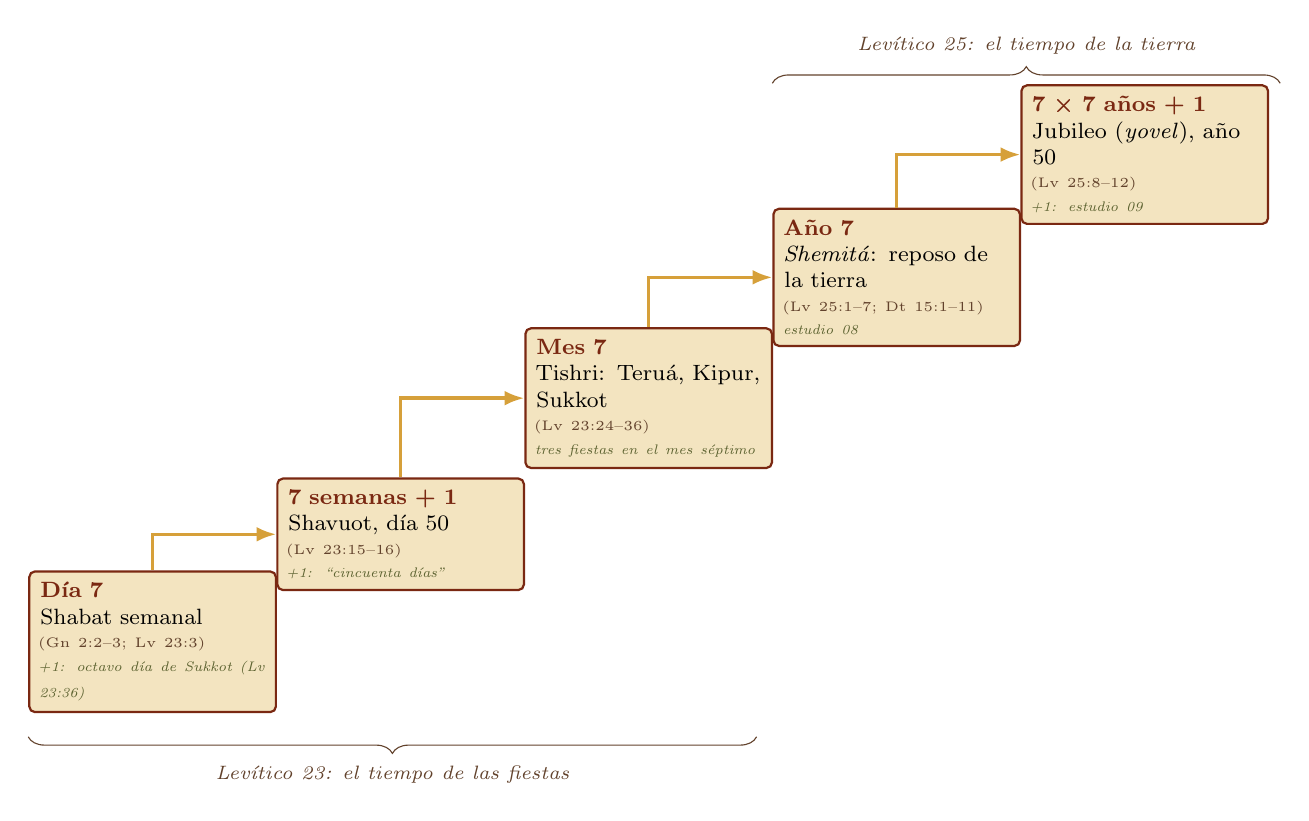
\begin{tikzpicture}[font=\footnotesize,x=1cm,y=1cm]
 \foreach \n/\t/\d/\r/\e in {0/{Día 7}/{Shabat semanal}/{Gn 2:2--3; Lv 23:3}/{+1: octavo día de Sukkot (Lv 23:36)}, 1/{7 semanas + 1}/{Shavuot, día 50}/{Lv 23:15--16}/{+1: ``cincuenta días''}, 2/{Mes 7}/{Tishri: Teruá, Kipur, Sukkot}/{Lv 23:24--36}/{tres fiestas en el mes séptimo}, 3/{Año 7}/{\emph{Shemitá}: reposo de la tierra}/{Lv 25:1--7; Dt 15:1--11}/{estudio 08}, 4/{7 × 7 años + 1}/{Jubileo (\emph{yovel}), año 50}/{Lv 25:8--12}/{+1: estudio 09}}{
   \node[draw=tierraroja,line width=0.8pt,fill=papiro,rounded corners=2pt,text width=2.85cm,align=left,anchor=south west,inner sep=4pt] (s\n) at (\n*3.15,\n*1.55) {\textbf{\textcolor{tierraroja}{\t}}\\ \d\\[-1pt] {\tiny\color{sepia}(\r)}\\[-1pt] {\tiny\itshape\color{oliva}\e}};}
 \foreach \a/\b in {0/1,1/2,2/3,3/4}{\draw[-{Latex[length=2.5mm]},mostaza,line width=1.2pt] (s\a.north) |- (s\b.west);}
 \draw[decorate,decoration={brace,amplitude=6pt,mirror},sepia] (0,-0.3) -- (9.25,-0.3) node[midway,below=7pt,font=\scriptsize\itshape,text=sepia] {Levítico 23: el tiempo de las fiestas};
 \draw[decorate,decoration={brace,amplitude=6pt},sepia] (9.45,8.0) -- (15.9,8.0) node[midway,above=7pt,font=\scriptsize\itshape,text=sepia] {Levítico 25: el tiempo de la tierra};
\end{tikzpicture}\par
{\footnotesize\color{sepia}\textit{Figura 5.} La escalera del siete. \textit{Nota.} Elaboración propia con la RVR1960. En verde oliva, el ``uno más'' de cada escala y los estudios de la serie que la desarrollan.}
\end{center}

En la escala del día, el séptimo es Shabat. En la de la semana, siete semanas ``cumplidas'' llevan al día cincuenta, Shavuot (Lv 23:15--16). En la del mes, el séptimo concentra tres solemnidades, el primero, el décimo y el decimoquinto de Tishri. En la del año, el séptimo es la \emph{shemitá}, en que ``la tierra tendrá descanso, reposo para el \SENOR'' (\heb{שַׁבַּת שַׁבָּתוֹן יִהְיֶה לָאָרֶץ}, Lv 25:4), con lo que la tierra recibe el mismo título que el día séptimo y que el día de las expiaciones. Y en la escala de la generación, ``siete semanas de años, siete veces siete años'' llevan al año cincuenta, el Jubileo, proclamado con trompeta ``el día de la expiación'' (Lv 25:8--10), cuando cada uno vuelve a su posesión. A esto se suma el siete interno de las fiestas: siete días de ázimos, siete de cabañas y siete días anuales de convocación santa.

El ``uno más'' merece atención, porque el octavo día de Sukkot, el día cincuenta de Shavuot y el año cincuenta del Jubileo quedan fuera del ciclo de siete y a la vez lo completan: son el comienzo de otro ciclo. La serie leerá en ese octavo día una figura del tiempo posterior al Milenio (§\ref{sec:serie}); el Nuevo Testamento, por su parte, asocia la resurrección con ``el primer día de la semana'', el día que sigue al séptimo (Mc 16:2; Jn 20:1, 19).

\begin{nota}[Precisión]
Los ciclos de Lv 25 vuelven en la historia de Israel: el cronista interpreta los setenta años del exilio como el tiempo en que ``la tierra hubo gozado de reposo'', los sábados de la tierra no guardados (2~Cr 36:21; cf. Lv 26:34--35), y Daniel recibe ``setenta semanas'' de años (Dn 9:24). El cálculo de 490 años de infidelidad a partir de 2~Cr 36:21 es tradicional (cf. \emph{Seder Olam}) pero no está explícito en el texto. La serie dedica a la \emph{shemitá} el estudio 08 y al Jubileo el estudio 09.
\end{nota}

%===================================================================
\section{Lectura filológica: el vocabulario del tiempo santo}\label{sec:filologia}

El vocabulario de Levítico 23 es preciso, y cada término nombra un aspecto distinto de la fiesta: la cita (\emph{moed}), la convocatoria (\emph{mikrá}), la peregrinación (\emph{jag}), el cese (\emph{shabat}, \emph{shabatón}), el recuerdo (\emph{zikarón}) y la permanencia (\emph{jukat olam}).

\begin{filologia}[\heb{מוֹעֵד} \emph{moed}, plural \heb{מוֹעֲדִים} \emph{moadim}]
\textbf{Raíz} \heb{יעד} (\emph{y-'-d}), ``fijar, citar, designar''. En nifal, ``encontrarse en el lugar y la hora convenidos'' (Am 3:3: ``¿Andarán dos juntos, si no estuvieren de acuerdo?''). \emph{Moed} es lo convenido: un \textbf{tiempo} señalado, un \textbf{lugar} de encuentro o una \textbf{asamblea} reunida.\par\smallskip
\textbf{Tiempo}: ``para las estaciones'' (\emph{lemoadim}, Gn 1:14; Sal 104:19); ``a su tiempo'' (\emph{bemoadó}, Nm 28:2); ``la visión tardará aún por un tiempo'' (\emph{lamoed}, Hab 2:3); ``tiempo, tiempos y la mitad de un tiempo'' (\emph{moed moadim vajetsi}, Dn 12:7).\par
\textbf{Lugar}: \heb{אֹהֶל מוֹעֵד} (\emph{óhel moed}), ``tabernáculo de reunión'': ``a la puerta del tabernáculo de reunión\ldots{} donde me reuniré con vosotros (\heb{אִוָּעֵד}, \emph{ivaed})'' (Éx 29:42). El tabernáculo es el \emph{moed} en el espacio; las fiestas, el \emph{moed} en el tiempo.\par
\textbf{En Lv 23}: ``las citas del \SENOR'' (\emph{moadé YHWH}, vv. 2, 4, 37, 44); ``mis citas'' (\emph{moaday}, v. 2); ``en su tiempo'' (\emph{bemoadam}, v. 4).\par
\textbf{LXX}: \grc{ἑορτή} (``fiesta'') en Lv 23:2; \grc{καιρός} (``tiempo oportuno'') en Gn 1:14; \grc{σκηνὴ τοῦ μαρτυρίου} (``tienda del testimonio'') para \emph{óhel moed}, leído desde \heb{עֵדוּת} (\emph{edut}, ``testimonio'').
\end{filologia}

La traducción ``fiestas solemnes'' es correcta, pero pierde lo que el término tiene de cita fijada por quien convoca. Por eso Lv 23:4 añade que se proclaman \emph{bemoadam}, ``en sus tiempos'': la fecha la fija quien convoca, no quien acude.

\begin{filologia}[\heb{מִקְרָא קֹדֶשׁ} \emph{mikrá kódesh}]
\textbf{Raíz} \heb{קרא} (\emph{k-r-'}), ``llamar, proclamar, leer en voz alta''. \emph{Mikrá} es ``lo llamado'': la \textbf{convocación} o asamblea reunida por un llamado (``el convocar asambleas'', \emph{keró mikrá}, Is 1:13; ``sus asambleas'', Is 4:5) y también la \textbf{lectura} pública: ``leían en el libro de la ley de Dios claramente\ldots{} de modo que entendiesen la lectura'' (\emph{bamikrá}, Neh 8:8). En hebreo rabínico, \emph{Mikrá} designa la Escritura misma.\par\smallskip
\textbf{En Lv 23}: once veces, conteo propio sobre el Códice de Leningrado (vv. 2, 3, 4, 7, 8, 21, 24, 27, 35, 36, 37); siempre con el verbo de la misma raíz: ``las cuales \emph{proclamaréis} (\heb{תִּקְרְאוּ}) como santas \emph{convocaciones}'' (vv. 2, 4, 37; cf. 21).\par
\textbf{LXX}: \grc{κλητὴ ἁγία}, ``llamada santa'' (Lv 23:2: \grc{ἃς καλέσετε αὐτὰς κλητὰς ἁγίας}).\par
\textbf{Precisión}: la explicación popular de \emph{mikrá} como ``ensayo'' (las fiestas como ensayos generales del plan de Dios; Chumney, 1994) es una \emph{analogía} homilética, no un significado del término. Lo que la palabra sí sostiene es la convocatoria pública y la lectura en voz alta.
\end{filologia}

\begin{filologia}[\heb{חַג} \emph{jag}]
\textbf{Raíz} \heb{חגג} (\emph{j-g-g}), ``celebrar una fiesta de peregrinación''; algunos léxicos proponen un sentido primario de ``girar, danzar en ronda'' (cf. Sal 107:27; 1~S 30:16), discutido (BDB; HALOT). Cognado del árabe \emph{ḥajj}, la peregrinación a La Meca.\par\smallskip
\textbf{Uso}: las tres fiestas de peregrinación: \emph{jag hamatsot}, \emph{jag hashavuot}, \emph{jag hasukot} (Dt 16:16); Éx 23:14: ``tres veces (\emph{regalim}) me celebraréis fiesta (\emph{tajog})''. En Lv 23, solo Matsot (v. 6) y Sukkot (vv. 34, 39, 41) se llaman \emph{jag}. Por metonimia, la víctima de la fiesta: ``el sebo de mi víctima'' (\emph{jelev jagí}, Éx 23:18).\par
\textbf{LXX y NT}: \grc{ἑορτή}; ``una fiesta de los judíos'' (Jn 5:1); ``celebremos la fiesta'' (\grc{ἑορτάζωμεν}, 1~Co 5:8).
\end{filologia}

\begin{filologia}[\heb{שַׁבָּת} \emph{shabat}, \heb{שַׁבָּתוֹן} \emph{shabatón}]
\textbf{Raíz} \heb{שׁבת} (\emph{sh-b-t}), ``cesar, detenerse'' (Gn 2:2; Jos 5:12). \emph{Shabat} es el día séptimo y, por extensión, la semana: ``siete semanas'' (\emph{sheva shabatot}, Lv 23:15).\par\smallskip
\emph{Shabatón}, forma intensiva o abstracta, ``reposo solemne'', se aplica a Teruá (Lv 23:24) y al primero y octavo de Sukkot (23:39). La combinación \heb{שַׁבַּת שַׁבָּתוֹן} (\emph{shabat shabatón}), ``sábado de solemne reposo'', se reserva para tres realidades: el Shabat semanal (Éx 31:15; 35:2; Lv 23:3), el día de las expiaciones (Lv 16:31; 23:32) y el año sabático de la tierra (Lv 25:4).\par
\textbf{LXX y NT}: \grc{σάββατα} (forma plural, que puede designar un solo sábado); \grc{ἀνάπαυσις}, ``reposo'', para \emph{shabatón} (Éx 16:23); \grc{σαββατισμός} (He 4:9).
\end{filologia}

\begin{filologia}[\heb{זִכָּרוֹן} \emph{zikarón}]
\textbf{Raíz} \heb{זכר} (\emph{z-k-r}), ``recordar''. \emph{Zikarón} es ``memorial'': lo que hace presente lo recordado.\par\smallskip
\textbf{Uso}: la Pascua: ``este día os será en memoria'' (\emph{lezikarón}, Éx 12:14); el día primero del mes séptimo: \heb{זִכְרוֹן תְּרוּעָה} (\emph{zijrón teruá}), ``una conmemoración al son de trompetas'' (Lv 23:24); las trompetas de plata ``os serán por memoria'' (Nm 10:10). En Éx 20:8, \emph{zajor}, ``acuérdate''.\par
\textbf{LXX y NT}: \grc{μνημόσυνον} (Éx 12:14); en la Cena, \grc{εἰς τὴν ἐμὴν ἀνάμνησιν}, ``en memoria de mí'' (Lc 22:19; 1~Co 11:24--25).
\end{filologia}

\begin{filologia}[\heb{חֻקַּת עוֹלָם} \emph{jukat olam}]
\textbf{Términos}: \heb{חֻקָּה} (\emph{jukká}), ``estatuto, ordenanza'' (raíz \emph{j-k-k}, ``grabar, inscribir''); \heb{עוֹלָם} (\emph{olam}), ``tiempo remoto, duración indefinida'', ``para siempre''.\par\smallskip
\textbf{En Lv 23}: cuatro veces, conteo propio sobre el Códice de Leningrado (vv. 14, 21, 31, 41), siempre con \heb{לְדֹרֹתֵיכֶם} (\emph{ledoroteijem}), ``por vuestras generaciones'', y tres veces con \heb{בְּכֹל מוֹשְׁבֹתֵיכֶם}, ``en dondequiera que habitéis'' (vv. 14, 21, 31; también v. 3, del Shabat).\par
\textbf{Precisión}: \emph{olam} indica permanencia sin plazo fijado por el texto; no siempre equivale a ``eterno'' en sentido metafísico. La misma fórmula califica el sacerdocio aarónico (Éx 29:9; 40:15) y prescripciones sacrificiales (Lv 3:17; 6:18). Quienes sostienen la vigencia de las fiestas se apoyan en ella; quienes leen Hebreos como cambio de sacerdocio y de ley (He 7:12; 8:13) responden que lo perpetuo puede cumplirse en una forma nueva. El término no zanja el debate por sí solo.
\end{filologia}

\begin{filologia}[\heb{מְלֶאכֶת עֲבֹדָה} \emph{melejet avodá} y \heb{כָּל־מְלָאכָה} \emph{kol melajá}]
\emph{Melajá} es la ``obra'' o el ``oficio'' (Gn 2:2); \emph{avodá}, el ``trabajo, servicio'' (y también el culto). \emph{Melejet avodá} se traduce ``trabajo de siervos'' (RVR1960) y designa la labor ordinaria de producción. Seis veces en Lv 23 (vv. 7, 8, 21, 25, 35, 36), frente a tres de \emph{kol melajá}, ``ningún trabajo'', para el Shabat y Kipur (vv. 3, 28, 31). Milgrom (2001) entiende la primera como ``trabajo laborioso'', que permite preparar la comida (cf. Éx 12:16). Conteos propios sobre el Códice de Leningrado.
\end{filologia}

El paso del hebreo al griego fija el vocabulario cristiano. La Septuaginta reduce a una sola palabra, \grc{ἑορτή}, los dos términos que el hebreo distingue (\emph{moed} y \emph{jag}), y el Nuevo Testamento hereda esa reducción:

\begin{center}
\begin{tikzpicture}[font=\footnotesize,node distance=0.55cm]
 \tikzset{c/.style={draw=tierraroja,line width=0.8pt,fill=papiro,rounded corners=3pt,text width=2.95cm,align=center,inner sep=4pt,minimum height=1.0cm}}
 \node[font=\small\bfseries,text=tierraroja] (h0) at (0,0) {Hebreo};
 \node[font=\small\bfseries,text=tierraroja] (l0) at (3.85,0) {Septuaginta};
 \node[font=\small\bfseries,text=tierraroja] (n0) at (7.7,0) {Nuevo Testamento};
 \node[font=\small\bfseries,text=tierraroja] (e0) at (11.55,0) {RVR1960};
 \foreach \y/\h/\l/\n/\e in {-1.15/{\heb{מוֹעֲדֵי יְהוָה}\\ \emph{moadé YHWH}}/{\grc{αἱ ἑορταὶ κυρίου}\\ (Lv 23:2)}/{\grc{ἑορτή}\\ (Jn 5:1; Col 2:16)}/{``fiestas solemnes''}, -2.45/{\heb{מִקְרָא קֹדֶשׁ}\\ \emph{mikrá kódesh}}/{\grc{κλητὴ ἁγία}\\ (Lv 23:2--4)}/{\grc{κλητοῖς ἁγίοις}\\ (Ro 1:7; 1 Co 1:2)}/{``santa convocación''}, -3.75/{\heb{חַג}\\ \emph{jag}}/{\grc{ἑορτή}\\ (Éx 23:14; Dt 16:16)}/{\grc{ἑορτάζωμεν}\\ (1 Co 5:8)}/{``fiesta solemne''}, -5.05/{\heb{שַׁבָּת} / \heb{שַׁבָּתוֹן}\\ \emph{shabat / shabatón}}/{\grc{σάββατα / ἀνάπαυσις}\\ (Éx 16:23; Lv 23:3)}/{\grc{σάββατον / σαββατισμός}\\ (Mc 2:27; He 4:9)}/{``día de reposo''}}{
   \node[c] (h) at (0,\y) {\h}; \node[c] (l) at (3.85,\y) {\l}; \node[c,fill=tierraroja!8] (n) at (7.7,\y) {\n}; \node[c,draw=mostaza,fill=white] (e) at (11.55,\y) {\e};
   \draw[-{Latex[length=2.5mm]},mostaza,line width=1.1pt] (h)--(l); \draw[-{Latex[length=2.5mm]},mostaza,line width=1.1pt] (l)--(n); \draw[-{Latex[length=2.5mm]},mostaza,line width=1.1pt] (n)--(e);}
\end{tikzpicture}\par
{\footnotesize\color{sepia}\textit{Figura 6.} Del hebreo al español: el vocabulario de las fiestas. \textit{Nota.} Elaboración propia con la BHS, la LXX (Rahlfs-Hanhart) y NA28. La coincidencia léxica entre \grc{κλητὴ ἁγία} y \grc{κλητοῖς ἁγίοις} es un dato; que Pablo aluda a Lv 23 al llamar a los creyentes ``llamados a ser santos'' es solo un eco posible.}
\end{center}

\subsection{Las fiestas como reloj profético: \emph{moed} y \emph{kairós}}
En mis presentaciones anteriores he sostenido que ``las fiestas son el reloj de los tiempos proféticos'', y el hilo que une esa afirmación con la filología es léxico. La Septuaginta traduce \emph{moadim} con \grc{καιροί}, ``tiempos oportunos'': las lumbreras sirven \grc{εἰς καιρούς} (Gn 1:14), la luna fue hecha \grc{εἰς καιρούς} (Sal 103:19 LXX [104:19]) y la Pascua se celebra ``a su tiempo'' (Nm 9:3). Cuando Pablo escribe ``acerca de los tiempos y de las ocasiones'' (\grc{περὶ τῶν χρόνων καὶ τῶν καιρῶν}, 1~Ts 5:1), o habla de ``la dispensación del cumplimiento de los tiempos'' (\grc{τοῦ πληρώματος τῶν καιρῶν}, Ef 1:10), usa la palabra con que su Biblia griega nombraba las citas de Dios; y en Col 2:16--17 llama a las fiestas ``sombra de lo que ha de venir''. Mi lectura es que Pablo lee los tiempos de Dios con el calendario de las fiestas, y que \emph{mikrá}, que Strong (H4744) glosa también como ``ensayo, repaso, lectura'', sería el ensayo público de lo que vendrá.

\begin{nota}[Precisión]
La equivalencia \emph{moed} = \grc{καιρός} es real en la Septuaginta, pero no exclusiva: \grc{καιρός} traduce también \heb{עֵת} (\emph{et}, ``tiempo'') y otras palabras, y en 1~Ts 5:1 la expresión ``tiempos y sazones'' procede más bien de Dn 2:21 (LXX y Teodoción). Que Pablo piense en el calendario festivo al usar \grc{καιροί} es una lectura posible, más clara en Col 2:16--17 que en 1~Ts 5:1. La glosa ``ensayo'' de Strong no figura en BDB ni en HALOT, que dan ``convocación'' y ``lectura''.
\end{nota}

%===================================================================
\section{Lectura textual: problemas de texto y de cómputo}\label{sec:textual}

\subsection{El doble encabezado de Lv 23:2 y 23:4}
El capítulo tiene dos títulos, ``las fiestas solemnes del \SENOR\ldots{} serán estas'' (v. 2) y ``estas son las fiestas solemnes del \SENOR'' (v. 4), y entre ambos está el Shabat. La crítica histórica ve aquí la huella de una edición: Milgrom (2001) y otros atribuyen los vv. 2b--3 a la mano de la escuela de santidad, que habría antepuesto el Shabat a un calendario de fiestas anuales que comenzaba en el v. 4. La lectura canónica ve, en cambio, un recurso del autor: el v. 2 anuncia todas las citas, el v. 3 coloca el Shabat como la primera y la que da el modelo, y el v. 4 retoma el título para pasar a las fiestas ``en sus tiempos'', las de fecha anual (Hartley, 1992; Wenham, 1979). Para el propósito de esta serie, ambas lecturas llegan al mismo resultado: el texto final presenta el Shabat como solemnidad del \SENOR{} y como cabeza del calendario.

\subsection{``El día siguiente del día de reposo''}
La fecha de la gavilla y, por ella, la de Shavuot dependen de una expresión ambigua: \heb{מִמָּחֳרַת הַשַּׁבָּת} (\emph{mimojorat hashabat}, Lv 23:11, 15--16). Si \emph{shabat} es el primer día de Matsot, que es día de reposo, la gavilla se ofrece el 16 de Abib; si es el sábado semanal, se ofrece el domingo que cae dentro de la semana de los ázimos. La Septuaginta traduce ``al día siguiente del primero'' (\grc{τῇ ἐπαύριον τῆς πρώτης}), y Josefo fecha la gavilla el 16 (\emph{Antigüedades} 3.250), como los fariseos y la Misná; los saduceos y boetusianos, según el Talmud (\emph{Menajot} 65a--66a), y después los caraítas, cuentan desde el domingo; Jubileos y Qumrán, desde el domingo posterior a la semana de los ázimos. La serie propone una tercera vía, el día siguiente al cruce del mar. Los estudios 03 y 04 examinan el problema con detalle.

\subsection{Otros puntos de cómputo}
Tres datos más dividen a los intérpretes. La hora de la Pascua, ``entre las dos tardes'' (\heb{בֵּין הָעַרְבָּיִם}, Éx 12:6; Lv 23:5), se entiende como el lapso entre la puesta del sol y la oscuridad (samaritanos, caraítas) o como la tarde, desde que el sol declina (Misná, \emph{Pesajim} 5:1; Josefo); el estudio 01 lo trata. El comienzo del día es explícito para Kipur, ``de tarde a tarde'' (Lv 23:32), y la práctica de Nehemías confirma que el Shabat comenzaba al oscurecer (Neh 13:19). El cómputo del mes, por último, depende de cómo se fije la luna nueva: por observación de la primera luna creciente (práctica antigua y caraíta) o por cálculo (calendario rabínico fijo).

\begin{nota}[Precisión textual]
El texto consonántico de Levítico 23 es estable: el Pentateuco Samaritano, la Septuaginta y los fragmentos de Levítico hallados en Qumrán no presentan variantes que alteren las fechas o las categorías del calendario. Las diferencias son de interpretación (\emph{mimojorat hashabat}, \emph{ben haarbáyim}) y de sistema de calendario (lunisolar o de 364 días), no de texto. La Septuaginta, al traducir ``del primero'' en Lv 23:11, refleja ya una interpretación y no un texto hebreo distinto. Sigo aquí el Texto Masorético.
\end{nota}

%===================================================================
\section{Lectura literaria: la forma del calendario}\label{sec:literaria}

\subsection{Cinco discursos y un marco}
La fórmula ``Habló el \SENOR{} a Moisés, diciendo'' divide el capítulo en cinco discursos. El primero contiene el Shabat y la Pascua con los ázimos; el segundo, la gavilla y las semanas; el tercero, el cuarto y el quinto corresponden a las tres solemnidades del mes séptimo. Un marco de títulos con \emph{moadé YHWH} encierra el conjunto: vv. 2 y 4 al comienzo, vv. 37 y 44 al final. Dentro del marco, dos cierres con ``Yo el \SENOR{} vuestro Dios'' (vv. 22 y 43) concluyen respectivamente la sección de primavera y la de otoño.

\begin{center}
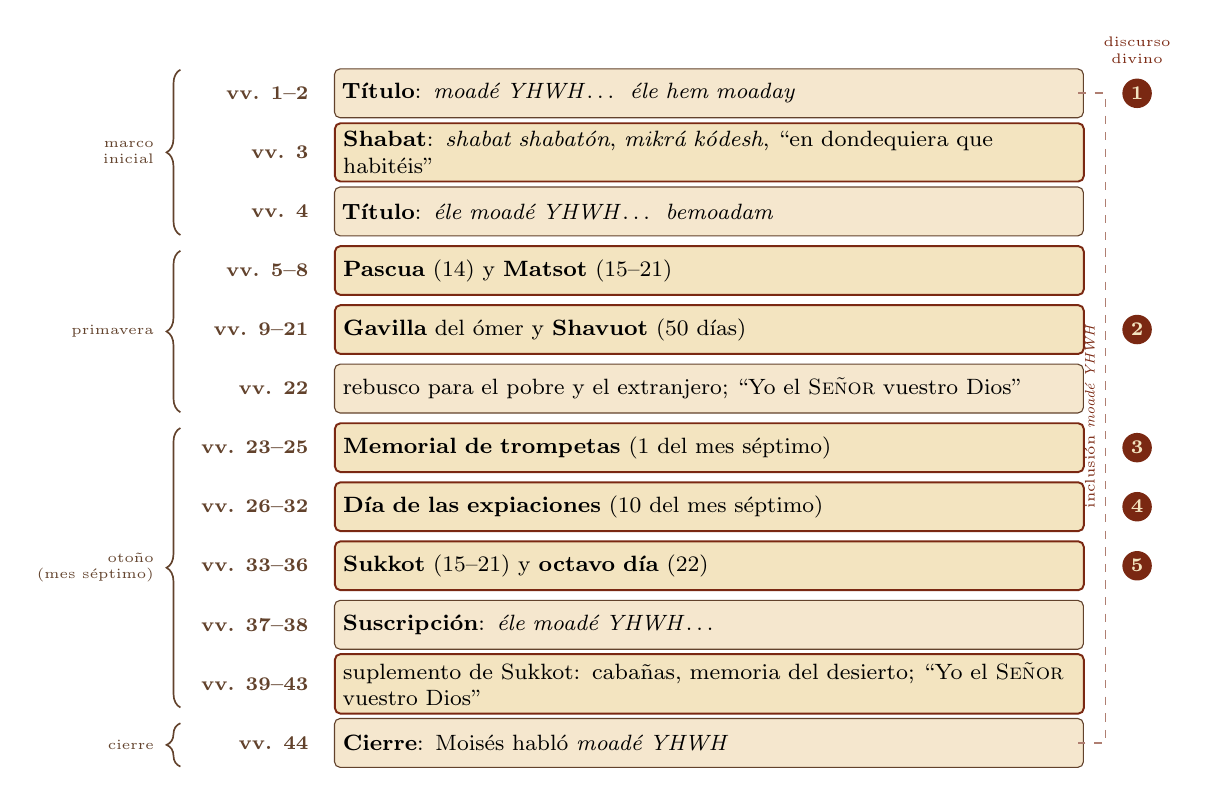
\begin{tikzpicture}[font=\footnotesize,x=1cm,y=1cm]
 \tikzset{b/.style={draw=tierraroja,line width=0.7pt,fill=papiro,rounded corners=2pt,minimum height=0.62cm,anchor=west,inner sep=3pt,align=left},
          f/.style={draw=sepia,fill=mostaza!25,rounded corners=2pt,minimum height=0.62cm,anchor=west,inner sep=3pt,align=left},
          d/.style={circle,fill=tierraroja,text=papiro,font=\scriptsize\bfseries,inner sep=1.5pt}}
 \foreach \y/\v/\t/\s in {0/{1--2}/{\textbf{Título}: \emph{moadé YHWH}\ldots{} \emph{éle hem moaday}}/f, -0.75/{3}/{\textbf{Shabat}: \emph{shabat shabatón}, \emph{mikrá kódesh}, ``en dondequiera que habitéis''}/b, -1.5/{4}/{\textbf{Título}: \emph{éle moadé YHWH}\ldots{} \emph{bemoadam}}/f, -2.25/{5--8}/{\textbf{Pascua} (14) y \textbf{Matsot} (15--21)}/b, -3.0/{9--21}/{\textbf{Gavilla} del ómer y \textbf{Shavuot} (50 días)}/b, -3.75/{22}/{rebusco para el pobre y el extranjero; ``Yo el \SENOR{} vuestro Dios''}/f, -4.5/{23--25}/{\textbf{Memorial de trompetas} (1 del mes séptimo)}/b, -5.25/{26--32}/{\textbf{Día de las expiaciones} (10 del mes séptimo)}/b, -6.0/{33--36}/{\textbf{Sukkot} (15--21) y \textbf{octavo día} (22)}/b, -6.75/{37--38}/{\textbf{Suscripción}: \emph{éle moadé YHWH}\ldots}/f, -7.5/{39--43}/{suplemento de Sukkot: cabañas, memoria del desierto; ``Yo el \SENOR{} vuestro Dios''}/b, -8.25/{44}/{\textbf{Cierre}: Moisés habló \emph{moadé YHWH}}/f}{
   \node[font=\scriptsize\bfseries,text=sepia,anchor=east] at (1.6,\y) {vv. \v};
   \node[\s,text width=9.3cm] at (1.8,\y) {\t};}
 \foreach \y/\n in {0/1,-2.25/1,-3.0/2,-4.5/3,-5.25/4,-6.0/5}{}
 \foreach \y/\n in {0.0/1,-3.0/2,-4.5/3,-5.25/4,-6.0/5}{\node[d] at (12.0,\y) {\n};}
 \node[font=\tiny,text=tierraroja,align=center] at (12.0,0.55) {discurso\\ divino};
 \draw[decorate,decoration={brace,amplitude=5pt,mirror},sepia,line width=0.6pt] (-0.15,0.3) -- (-0.15,-1.8) node[midway,left=6pt,font=\tiny,align=right,text=sepia] {marco\\ inicial};
 \draw[decorate,decoration={brace,amplitude=5pt,mirror},sepia,line width=0.6pt] (-0.15,-2.0) -- (-0.15,-4.05) node[midway,left=6pt,font=\tiny,align=right,text=sepia] {primavera};
 \draw[decorate,decoration={brace,amplitude=5pt,mirror},sepia,line width=0.6pt] (-0.15,-4.25) -- (-0.15,-7.8) node[midway,left=6pt,font=\tiny,align=right,text=sepia] {otoño\\ (mes séptimo)};
 \draw[decorate,decoration={brace,amplitude=5pt,mirror},sepia,line width=0.6pt] (-0.15,-8.0) -- (-0.15,-8.55) node[midway,left=6pt,font=\tiny,align=right,text=sepia] {cierre};
 \draw[tierraroja!60,dashed,line width=0.6pt] (11.25,0) -- (11.6,0) -- (11.6,-8.25) -- (11.25,-8.25);
 \node[font=\tiny,text=tierraroja,rotate=90] at (11.4,-4.1) {inclusión \emph{moadé YHWH}};
\end{tikzpicture}\par
{\footnotesize\color{sepia}\textit{Figura 7.} Estructura literaria de Levítico 23. \textit{Nota.} Elaboración propia. En mostaza, los títulos y fórmulas de marco; los círculos numerados señalan los cinco ``Habló el \SENOR{} a Moisés'' (vv. 1, 9, 23, 26, 33).}
\end{center}

\subsection{Las fórmulas repetidas}
El capítulo repite un pequeño repertorio de fórmulas, y contarlas muestra el peso que el texto da a cada idea:

\begin{center}\small\renewcommand{\arraystretch}{1.18}
\begin{tabular}{@{}L{4.6cm}L{4.1cm}L{1.3cm}L{5.0cm}@{}}
\toprule
\textbf{Fórmula} & \textbf{Hebreo} & \textbf{Veces} & \textbf{Versículos} \\ \midrule
``Habló el \SENOR{} a Moisés'' & \heb{וַיְדַבֵּר יְהוָה אֶל־מֹשֶׁה} & 5 & 1, 9, 23, 26, 33 \\
``Habla a los hijos de Israel'' & \heb{דַּבֵּר אֶל־בְּנֵי יִשְׂרָאֵל} & 4 & 2, 10, 24, 34 \\
``fiestas solemnes'' (\emph{moed}) & \heb{מוֹעֲדֵי יְהוָה} y formas & 6 & 2 (2×), 4 (2×), 37, 44 \\
``santa convocación'' & \heb{מִקְרָא קֹדֶשׁ} & 11 & 2, 3, 4, 7, 8, 21, 24, 27, 35, 36, 37 \\
``ningún trabajo de siervos'' & \heb{כָּל־מְלֶאכֶת עֲבֹדָה לֹא תַעֲשׂוּ} & 6 & 7, 8, 21, 25, 35, 36 \\
``ningún trabajo'' & \heb{כָּל־מְלָאכָה לֹא תַעֲשׂוּ} & 3 & 3, 28, 31 \\
``estatuto perpetuo'' & \heb{חֻקַּת עוֹלָם} & 4 & 14, 21, 31, 41 \\
``por vuestras generaciones'' & \heb{לְדֹרֹתֵיכֶם} & 4 & 14, 21, 31, 41 \\
``en dondequiera que habitéis'' & \heb{בְּכֹל מוֹשְׁבֹתֵיכֶם} & 4 & 3, 14, 21, 31 \\
``reposo solemne'' (\emph{shabatón}) & \heb{שַׁבָּתוֹן} & 5 & 3, 24, 32, 39 (2×) \\
``Yo el \SENOR{} vuestro Dios'' & \heb{אֲנִי יְהוָה אֱלֹהֵיכֶם} & 2 & 22, 43 \\
\bottomrule
\end{tabular}\par
{\footnotesize\color{sepia}\textit{Tabla 7.} Fórmulas de Levítico 23. \textit{Nota.} Conteo propio sobre el Códice de Leningrado (base de la BHS), con variantes de grafía plena y defectiva (\emph{moshvoteijem}, v. 3) y con conjunción inicial (v. 28). La fórmula del v. 41 dice ``por vuestras generaciones'' sin ``en dondequiera que habitéis''; el v. 17 dice ``de vuestras habitaciones'' (\emph{mimoshvoteijem}), con otro sentido.}
\end{center}

Sin atribuir a las cifras más de lo que dicen, las palabras más repetidas son las de la convocatoria (\emph{mikrá}, once veces) y las del reposo (seis más tres prohibiciones de trabajo y cinco \emph{shabatón}); el capítulo legisla menos sobre qué hacer que sobre cuándo detenerse y reunirse. Las fórmulas de permanencia se concentran en cuatro lugares: la gavilla (v. 14), Shavuot (v. 21), Kipur (v. 31) y Sukkot (v. 41).

\subsection{Levítico 23 en su libro}
Levítico 23 pertenece a la sección que la crítica llama ``Código de santidad'' (Lv 17--26), dominada por el estribillo ``Santos seréis, porque santo soy yo el \SENOR{} vuestro Dios'' (19:2). La sección avanza en círculos concéntricos de santidad: el pueblo (Lv 18--20), los sacerdotes y las ofrendas (21--22), el tiempo (23), el santuario con su lámpara y su pan ``cada día de reposo'' (24:1--9) y la tierra con sus años sabáticos (25). El calendario queda así entre la santidad de las personas y la santidad de la tierra. Dos veces la sección resume su ética con la misma pareja, ``Mis días de reposo guardaréis, y mi santuario tendréis en reverencia'' (19:30; 26:2): el tiempo santo y el espacio santo van juntos.

\subsection{Ecos intrabíblicos}
El calendario de Levítico 23 dialoga con la creación y con el éxodo. Con la creación, porque los \emph{moadim} de Lv 23:2 son los que las lumbreras de Gn 1:14 ``señalan'' y porque el Shabat de Lv 23:3 retoma el día séptimo de Gn 2:1--3, de modo que lo que Dios hizo al principio se convierte en ritmo para su pueblo. Con el éxodo, porque Pascua y Matsot remiten a Éx 12 y Sukkot a la vida en cabañas en el desierto (Lv 23:43). Dialoga también con la historia posterior de Israel: Josué celebra la Pascua en Gilgal al entrar en la tierra (Jos 5:10--12); Salomón dedica el templo en la fiesta del mes séptimo (1~R 8:2); Ezequías y Josías restauran la Pascua (2~Cr 30; 35); Esdras y Nehemías leen la Ley y celebran Sukkot ``como está escrito'' (Esd 3:4; Neh 8:13--18). Una y otra vez la reforma comienza volviendo al calendario.

%===================================================================
\section{Memorial, figura y esperanza: la lectura de la serie}\label{sec:serie}

La serie lee cada fiesta con un marco propio. Lo expongo aquí con sus textos de apoyo y agrego, separadas, las precisiones que el texto bíblico y la historia piden.

\subsection{La tabla maestra: dos rieles paralelos}
La serie lee el tránsito de Israel desde el cautiverio hasta la Tierra Prometida como figura del camino de la Iglesia (1~Co 10:11). Cada fiesta es \destacar{memorial} de un hito de Israel y \destacar{figura} de un hito del plan de salvación. La figura 8 lo dibuja como dos rieles que corren en paralelo, unidos por las estaciones del calendario; los conectores distinguen lo que el texto dice expresamente de lo que la serie lee como tipología.

\begin{center}
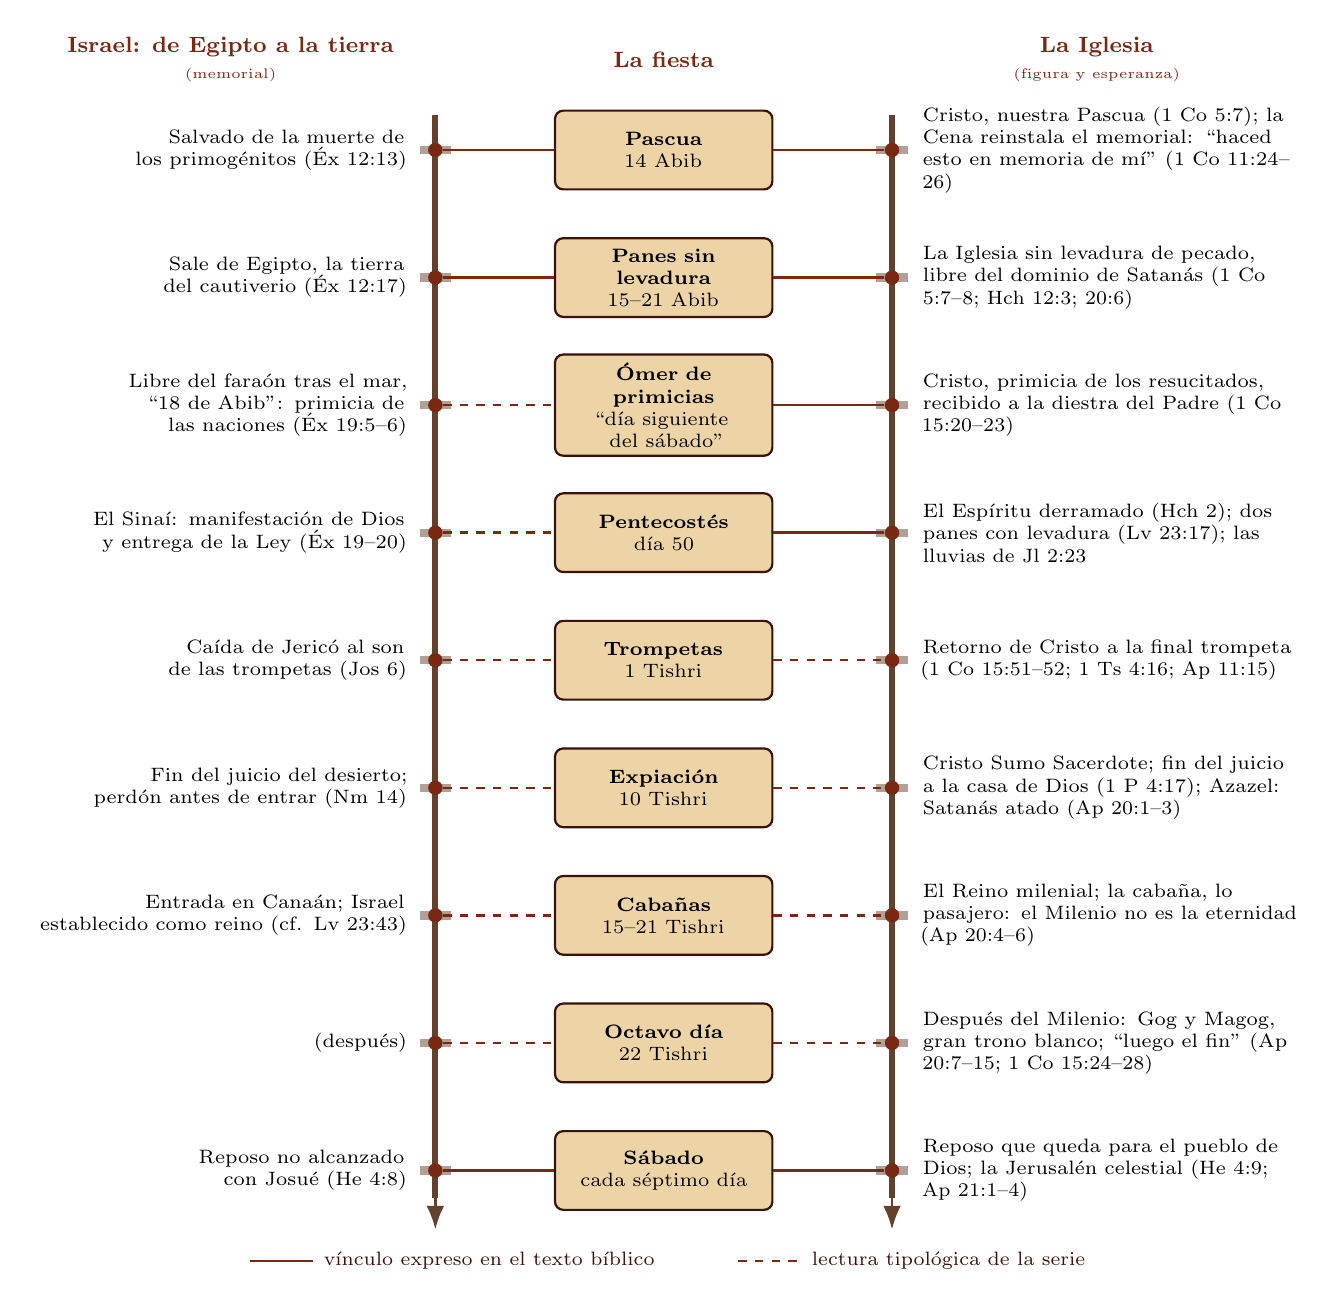
\begin{tikzpicture}[x=1cm,y=1cm,font=\scriptsize]
 \def\dy{1.62}
 \tikzset{f/.style={draw=caferojizo,line width=0.8pt,fill=mostaza!45,rounded corners=3pt,text width=2.55cm,align=center,inner sep=3pt,minimum height=1.0cm},
          L/.style={text width=4.75cm,align=right,anchor=east,inner sep=1pt},
          R/.style={text width=4.75cm,align=left,anchor=west,inner sep=1pt},
          ex/.style={tierraroja,line width=0.9pt}, ty/.style={tierraroja,line width=0.9pt,dashed}}
 % encabezados
 \node[font=\footnotesize\bfseries,text=tierraroja,align=center] at (2.75,1.15) {Israel: de Egipto a la tierra\\ \tiny\mdseries (memorial)};
 \node[font=\footnotesize\bfseries,text=tierraroja,align=center] at (8.25,1.15) {La fiesta};
 \node[font=\footnotesize\bfseries,text=tierraroja,align=center] at (13.75,1.15) {La Iglesia\\ \tiny\mdseries (figura y esperanza)};
 % rieles
 \draw[sepia,line width=2.2pt] (5.35,0.45) -- (5.35,-8*\dy-0.35);
 \draw[sepia,line width=2.2pt] (11.15,0.45) -- (11.15,-8*\dy-0.35);
 \foreach \k in {0,...,8}{\draw[sepia!50,line width=3pt] (5.15,-\k*\dy) -- (5.55,-\k*\dy); \draw[sepia!50,line width=3pt] (10.95,-\k*\dy) -- (11.35,-\k*\dy);}
 \draw[-{Latex[length=3mm]},sepia,line width=1pt] (5.35,-8*\dy-0.35) -- (5.35,-8*\dy-0.75);
 \draw[-{Latex[length=3mm]},sepia,line width=1pt] (11.15,-8*\dy-0.35) -- (11.15,-8*\dy-0.75);
 \foreach \k/\fa/\la/\ra/\cl/\cr in {
   0/{\textbf{Pascua}\\ 14 Abib}/{Salvado de la muerte de los primogénitos (Éx 12:13)}/{Cristo, nuestra Pascua (1 Co 5:7); la Cena reinstala el memorial: ``haced esto en memoria de mí'' (1 Co 11:24--26)}/ex/ex,
   1/{\textbf{Panes sin levadura}\\ 15--21 Abib}/{Sale de Egipto, la tierra del cautiverio (Éx 12:17)}/{La Iglesia sin levadura de pecado, libre del dominio de Satanás (1 Co 5:7--8; Hch 12:3; 20:6)}/ex/ex,
   2/{\textbf{Ómer de primicias}\\ ``día siguiente del sábado''}/{Libre del faraón tras el mar, ``18 de Abib'': primicia de las naciones (Éx 19:5--6)}/{Cristo, primicia de los resucitados, recibido a la diestra del Padre (1 Co 15:20--23)}/ty/ex,
   3/{\textbf{Pentecostés}\\ día 50}/{El Sinaí: manifestación de Dios y entrega de la Ley (Éx 19--20)}/{El Espíritu derramado (Hch 2); dos panes con levadura (Lv 23:17); las lluvias de Jl 2:23}/ty/ex,
   4/{\textbf{Trompetas}\\ 1 Tishri}/{Caída de Jericó al son de las trompetas (Jos 6)}/{Retorno de Cristo a la final trompeta (1 Co 15:51--52; 1 Ts 4:16; Ap 11:15)}/ty/ty,
   5/{\textbf{Expiación}\\ 10 Tishri}/{Fin del juicio del desierto; perdón antes de entrar (Nm 14)}/{Cristo Sumo Sacerdote; fin del juicio a la casa de Dios (1 P 4:17); Azazel: Satanás atado (Ap 20:1--3)}/ty/ty,
   6/{\textbf{Cabañas}\\ 15--21 Tishri}/{Entrada en Canaán; Israel establecido como reino (cf. Lv 23:43)}/{El Reino milenial; la cabaña, lo pasajero: el Milenio no es la eternidad (Ap 20:4--6)}/ty/ty,
   7/{\textbf{Octavo día}\\ 22 Tishri}/{(después)}/{Después del Milenio: Gog y Magog, gran trono blanco; ``luego el fin'' (Ap 20:7--15; 1 Co 15:24--28)}/ty/ty,
   8/{\textbf{Sábado}\\ cada séptimo día}/{Reposo no alcanzado con Josué (He 4:8)}/{Reposo que queda para el pueblo de Dios; la Jerusalén celestial (He 4:9; Ap 21:1--4)}/ex/ex}{
   \node[f] (f\k) at (8.25,-\k*\dy) {\fa};
   \node[L] at (5.0,-\k*\dy) {\la};
   \node[R] at (11.5,-\k*\dy) {\ra};
   \fill[tierraroja] (5.35,-\k*\dy) circle (2.6pt); \fill[tierraroja] (11.15,-\k*\dy) circle (2.6pt);
   \draw[\cl] (5.45,-\k*\dy) -- (f\k.west);
   \draw[\cr] (f\k.east) -- (11.05,-\k*\dy);}
 % leyenda
 \draw[tierraroja,line width=0.9pt] (3.0,-8*\dy-1.15) -- (3.8,-8*\dy-1.15) node[right,text=caferojizo] {vínculo expreso en el texto bíblico};
 \draw[tierraroja,line width=0.9pt,dashed] (9.2,-8*\dy-1.15) -- (10.0,-8*\dy-1.15) node[right,text=caferojizo] {lectura tipológica de la serie};
\end{tikzpicture}\par
{\footnotesize\color{sepia}\textit{Figura 8.} La tabla maestra de la serie: Israel y la Iglesia en dos rieles paralelos. \textit{Nota.} Elaboración propia. En Expiación, Hebreos sí relaciona expresamente el día de las expiaciones con el sacerdocio de Cristo (He 9:7--12); lo tipológico es el resto del contenido asignado por la serie. En Cabañas, Lv 23:43 vincula expresamente la fiesta con la vida en cabañas en el desierto, no con la entrada en Canaán.}
\end{center}

El esquema tiene una lógica interna. Israel es salvado de la muerte (Pascua), sale de Egipto (Ázimos), queda libre del faraón como primicia de las naciones (ómer), recibe la Ley y la presencia de Dios en el Sinaí (Pentecostés), entra en la tierra al son de las trompetas de Jericó (Trompetas) con el juicio del desierto concluido (Expiación), y se establece como reino (Cabañas). Del mismo modo, la Iglesia es redimida por Cristo, nuestra Pascua; vive sin la levadura del pecado; tiene en Cristo resucitado la primicia de su propia resurrección; recibe el Espíritu en Pentecostés; espera la última trompeta, el fin del juicio que comienza ``por la casa de Dios'' y el Reino; y, después del Milenio y del juicio final (el octavo día), alcanza el reposo definitivo de la Jerusalén celestial (el Sábado).

\subsection{Precisiones a la tabla maestra}
La serie expone su lectura como una tesis argumentada, y cada estudio la examinará fiesta por fiesta. Desde ahora fijo cuatro precisiones.

\begin{nota}[Precisión 1: lo explícito y lo tipológico]
La Torá vincula expresamente la Pascua con la noche de los primogénitos (Éx 12:13, 27), los Ázimos con la salida de Egipto (Éx 12:17, 39) y Sukkot con las cabañas del desierto (Lv 23:43). Para el ómer y Shavuot no da memorial histórico: la asociación de Shavuot con el Sinaí aparece en el Segundo Templo (Jubileos 6:17--21) y en el Talmud (\emph{Shabat} 86b), apoyada en Éx 19:1 (``en el mes tercero''). Los vínculos Trompetas--Jericó, Expiación--fin del juicio del desierto y Cabañas--entrada a Canaán no están en el texto. Además, según Jos 5:10--12, Israel celebró la Pascua en Gilgal el 14 del mes primero, poco antes de la toma de Jericó (Jos 6), de modo que la caída de la ciudad ocurrió en primavera y no en el mes séptimo. La lectura de la serie es tipológica, no cronológica.
\end{nota}

\begin{nota}[Precisión 2: la fecha del éxodo]
La cronología interna de la Biblia permite fechar la salida de Egipto: ``en el año cuatrocientos ochenta después que los hijos de Israel salieron de Egipto'' Salomón comenzó el templo (1~R 6:1), hacia 967/966 a.\,e.\,c., lo que sitúa el éxodo hacia 1446 a.\,e.\,c. (la llamada fecha temprana). Muchos historiadores, a partir de la ciudad de ``Ramesés'' (Éx 1:11) y de la arqueología de Canaán, proponen una fecha tardía, hacia 1260 a.\,e.\,c. (Sarna, 1991; Propp, 1999).
\end{nota}

\begin{nota}[Precisión 3: el cruce del mar y el ``18 de Abib'']
La serie reconstruye el itinerario de Nm 33:5--8 (Ramesés, Sucot, Etam, Pi-hahirot) y sitúa el cruce del mar el tercer día, 17 de Abib, de modo que el 18 Israel queda libre del faraón como primicia de las naciones. El texto bíblico no fecha el cruce. La tradición rabínica lo sitúa el 21 de Nisán, séptimo día de Matsot (\emph{Seder Olam Rabá} 5; Rashi a Éx 14:5), y por eso se lee el cántico del mar (Éx 15) en ese día. Las dos reconstrucciones son inferencias.
\end{nota}

\begin{nota}[Precisión 4: los textos de vigencia]
La serie reúne los textos que muestran a la Iglesia apostólica en el calendario de las fiestas: Lc 23:56; Hch 2:1; 12:3; 20:6, 16; 27:9; 1~Co 5:8; 16:8; Jn 7; Col 2:16--17. Unos son marcas de tiempo narrativas (Hch 12:3; 20:6; 27:9), que muestran que el calendario judío ordenaba la vida de los primeros creyentes; otros son textos teológicos (1~Co 5:7--8; Col 2:16--17). Si de ellos se sigue una obligación para las iglesias gentiles es justamente lo que se discute. Sobre 1~Co 5:8 (``celebremos la fiesta''), Fee (1987) lo lee como metáfora de toda la vida cristiana; la serie, como referencia a la fiesta literal. Ambos reconocen que Pablo escribe pensando en la Pascua y los ázimos.
\end{nota}

%===================================================================
\section{¿Para quién son las fiestas?}\label{sec:paraquien}

En la presentación con que abrí esta serie planteé una pregunta previa a todas las demás: si las fiestas son ``de Israel'', ¿quién es Israel? La respuesta recorre la historia del pueblo desde Jacob hasta el nuevo pacto. Expongo aquí esa lectura y marco lo que el texto sostiene.

\subsection{Cuatro ``mitos'' y una historia de amor}
La presentación parte de una pregunta abierta (¿quién es Israel: los judíos, un país, Jacob, la Iglesia, los cristianos?) y enfrenta cuatro afirmaciones corrientes que llamé ``mitos'': que los judíos fueron \emph{el} pueblo escogido, que la Ley fue dada solo a los judíos, que las festividades que Jesús celebró eran para los judíos y que la ley judía quedó clavada en la cruz. La respuesta tiene cinco conclusiones: (1) Jacob bendice a Efraín con heredad, nombre y ``multitud de naciones''; (2) la división de Israel fue voluntad de Dios; (3) el Mesías viene por las ovejas esparcidas de la casa de Israel; (4) el Mesías tiene que morir para casarse de nuevo con su novia Israel; y (5) el nuevo pacto es con la casa de Israel y con la casa de Judá. Los apartados siguientes recorren los textos en que se apoya.

\subsection{Israel, Efraín y la ``multitud de naciones''}
Israel es primero el nombre de un hombre, Jacob (Gn 32:28), y luego el de sus doce tribus. Al bendecir a los hijos de José, Jacob anuncia del menor:

\hebverso{וְאוּלָם אָחִיו הַקָּטֹן יִגְדַּל מִמֶּנּוּ וְזַרְעוֹ יִהְיֶה מְלֹא־הַגּוֹיִם}
\begin{cita}Pero su hermano menor será más grande que él, y su descendencia formará multitud de naciones.\fuente{(Gn 48:19)}\end{cita}

La expresión \emph{meló hagoyim}, ``plenitud de las naciones'', reaparece con su equivalente griego en Pablo: ``ha acontecido a Israel endurecimiento en parte, hasta que haya entrado la plenitud de los gentiles'' (\grc{τὸ πλήρωμα τῶν ἐθνῶν}, Ro 11:25). La historia de Efraín, cabeza del reino del norte, termina en dispersión: Asiria deporta a Israel (2~R 17:6, 23) y Oseas anuncia que será ``Lo-ammi'', ``no pueblo mío'' (Os 1:9), con una promesa: ``en el lugar en donde les fue dicho: Vosotros no sois pueblo mío, les será dicho: Sois hijos del Dios viviente'' (Os 1:10 [2:1]). Ezequiel ve las dos varas, Judá y Efraín, unidas en una sola mano (Ez 37:15--22). La división misma fue obra de Dios, y de ahí arranca el argumento. El profeta Ahías rasga su capa en doce pedazos y dice a Jeroboam: ``Toma para ti los diez pedazos; porque así dijo el \SENOR{} Dios de Israel: He aquí que yo rompo el reino de la mano de Salomón, y a ti te daré diez tribus'' (1~R 11:31); y cuando Roboam quiere recuperar el norte por la fuerza, Dios lo detiene: ``esto lo he hecho yo'' (1~R 12:24). La dispersión estaba anunciada en el pacto (Dt 28:64), y el pacto mismo incluía a los ausentes: ``no solamente con vosotros hago yo este pacto\ldots{} sino con los que están aquí presentes hoy\ldots{} y con los que no están aquí hoy con nosotros'' (Dt 29:14--15), con la promesa del regreso (Dt 30:1--5; Jer 31:1--3).

\subsection{Las ovejas perdidas y los dispersos}
Jesús define su misión con el lenguaje de esa dispersión: ``No soy enviado sino a las ovejas perdidas de la casa de Israel'' (Mt 15:24; cf. 10:6), y anuncia: ``También tengo otras ovejas que no son de este redil\ldots{} y habrá un rebaño, y un pastor'' (Jn 10:16). Juan explica que Jesús había de morir ``no solamente por la nación, sino también para congregar en uno a los hijos de Dios que estaban dispersos'' (Jn 11:52). Santiago escribe ``a las doce tribus que están en la dispersión'' (Stg 1:1), y Pedro ``a los expatriados de la dispersión'' en Asia Menor (1~P 1:1), a creyentes que, por lo que dice después, venían en buena parte del paganismo (1~P 1:18; 4:3).

El paso que cierra el argumento lo da Pablo al aplicar el texto de Oseas sobre el Israel disperso a los gentiles llamados en Cristo: ``a nosotros, no sólo de los judíos, sino también de los gentiles\ldots{} Como también en Oseas dice: Llamaré pueblo mío al que no era mi pueblo'' (Ro 9:24--25). Para Pablo, la restauración de Israel y la entrada de las naciones forman un solo movimiento.

Los profetas ya habían usado la imagen del rebaño: ``Ovejas perdidas fueron mi pueblo; sus pastores las hicieron errar'' (Jer 50:6; cf. 50:17; 23:3; Mi 2:12; Ez 34:12--15), y Dios mismo prometió ser para los dispersos ``un pequeño santuario en las tierras adonde lleguen'' (Ez 11:16). Cuando Jesús anuncia que se irá adonde no lo hallarán, sus oyentes preguntan: ``¿Se irá a los dispersos entre los griegos?'' (Jn 7:35).

\subsection{El olivo y la ciudadanía de Israel}
Pablo usa dos imágenes para describir el lugar de los gentiles. La primera es el olivo (Ro 11:16--27): la raíz es santa; algunas ramas naturales fueron desgajadas por incredulidad; ramas de olivo silvestre fueron injertadas ``y hechas participantes de la raíz y de la rica savia del olivo''; las ramas naturales pueden ser injertadas de nuevo, ``y luego todo Israel será salvo'' (11:26). La segunda es la ciudadanía: los gentiles estaban ``alejados de la ciudadanía de Israel y ajenos a los pactos de la promesa'' (Ef 2:12), pero en Cristo ``ya no sois extranjeros ni advenedizos, sino conciudadanos de los santos, y miembros de la familia de Dios'' (2:19).

\begin{center}
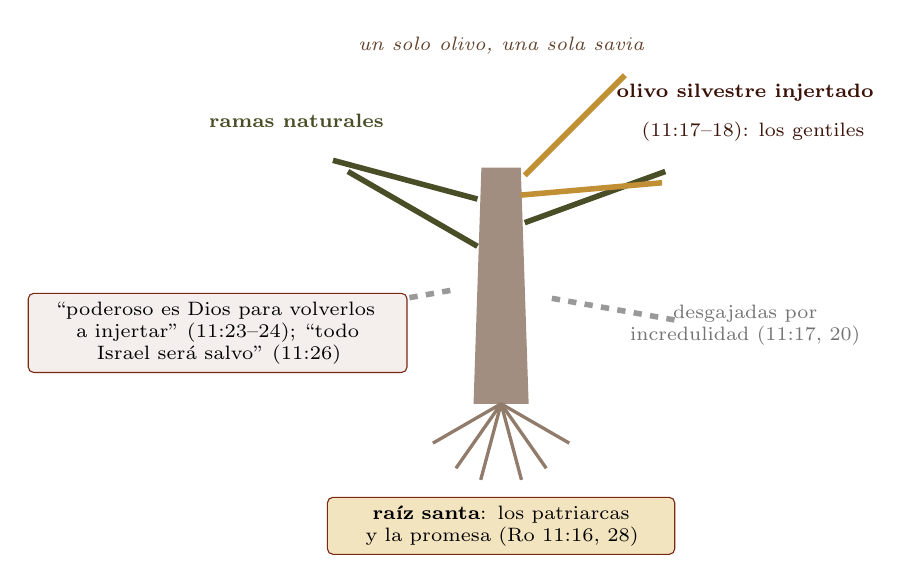
\begin{tikzpicture}[font=\scriptsize]
 \fill[sepia!60] (-0.35,0) -- (-0.25,3.0) -- (0.25,3.0) -- (0.35,0) -- cycle;
 \foreach \a in {-60,-35,-15,15,35,60}{\draw[sepia!70,line width=1.2pt] (0,0) -- (\a-90:1.0);}
 \node[draw=tierraroja,fill=papiro,rounded corners=2pt,text width=4.2cm,align=center,inner sep=3pt] at (0,-1.55) {\textbf{raíz santa}: los patriarcas y la promesa (Ro 11:16, 28)};
 \foreach \x/\y/\a in {-0.3/2.0/150,-0.3/2.6/165,0.3/2.3/20}{\draw[oliva!80!black,line width=2pt] (\x,\y) -- ++(\a:1.9);}
 \node[text=oliva!80!black,align=center,font=\scriptsize\bfseries] at (-2.6,3.6) {ramas naturales};
 \foreach \x/\y/\a in {0.3/1.4/-10,-0.3/1.5/190}{\draw[black!40,line width=2pt,dashed] (\x,\y) ++(\a:0.35) -- ++(\a:1.6);}
 \node[text=black!55,align=center] at (3.1,1.0) {desgajadas por\\ incredulidad (11:17, 20)};
 \foreach \x/\y/\a in {0.3/2.9/45,0.25/2.65/5}{\draw[mostaza!90!black,line width=2pt] (\x,\y) -- ++(\a:1.8);}
 \node[text=caferojizo,align=center,font=\scriptsize\bfseries] at (3.1,3.95) {olivo silvestre injertado};
 \node[text=caferojizo,align=center] at (3.2,3.45) {(11:17--18): los gentiles};
 \node[draw=tierraroja,fill=tierraroja!8,rounded corners=2pt,text width=4.6cm,align=center,inner sep=3pt] at (-3.6,0.9) {``poderoso es Dios para volverlos a injertar'' (11:23--24); ``todo Israel será salvo'' (11:26)};
 \node[font=\scriptsize\itshape,text=sepia] at (0,4.55) {un solo olivo, una sola savia};
\end{tikzpicture}\par
{\footnotesize\color{sepia}\textit{Figura 9.} El olivo de Romanos 11. \textit{Nota.} Elaboración propia, esquemática.}
\end{center}

\subsection{Una historia de amor}
En la presentación leí el conjunto como una historia conyugal. Dios da a la Israel del norte ``carta de repudio'' (Jer 3:8; cf. 3:1), y la Ley impedía que la repudiada volviera a su primer marido (Dt 24:1--4). La salida la abre la muerte: ``la mujer casada está sujeta por la ley al marido mientras éste vive; pero si el marido muere, ella queda libre'' (Ro 7:2); ``así también vosotros\ldots{} habéis muerto a la ley mediante el cuerpo de Cristo, para que seáis de otro, del que resucitó de los muertos'' (7:4). El Mesías muere para que la novia pueda volver a casarse, y la historia termina en ``las bodas del Cordero'' (Ap 19:7--9). El nuevo pacto es, en esta lectura, una renovación de votos que Dios hace con la casa de Israel y con la casa de Judá, y cuyo contenido es la \emph{torá} escrita en el corazón (Jer 31:33). \emph{Torá} (\heb{תּוֹרָה}, de \emph{y-r-h}, ``apuntar, enseñar'') es ``instrucción, dirección'' antes que ``código legal''.

\begin{nota}[Precisión]
La lectura conyugal tiene bases sólidas: el matrimonio de Dios con Israel es imagen profética (Os 2; Jer 2:2; 3; Ez 16) y la Iglesia aparece como esposa de Cristo (Ef 5:25--32; Ap 19:7; 21:2). La aplicación de Ro 7:1--4 a la restauración de la Israel repudiada de Jer 3 es, en cambio, lectura de la serie: en Romanos, quien ``muere'' a la ley es el creyente, y la ilustración matrimonial sirve para explicar su liberación de la ley como poder que condena (Moo, 1996; Dunn, 1998). Las dos lecturas coinciden en que la muerte de Cristo crea una relación nueva y fecunda (``para que llevemos fruto para Dios'', Ro 7:4).
\end{nota}

\subsection{Una misma ley para el natural y el extranjero}
La Torá ya preveía la incorporación del extranjero a las fiestas. Para la Pascua: ``Mas si algún extranjero morare contigo, y quisiere celebrar la pascua para el \SENOR, séale circuncidado todo varón, y entonces la celebrará, y será como uno de vuestra nación\ldots{} La misma ley será para el natural, y para el extranjero que habitare entre vosotros'' (Éx 12:48--49; cf. Nm 15:15--16). Isaías abre el Shabat y el monte santo a los extranjeros que ``abracen mi pacto'' (Is 56:6--7), y Zacarías ve a las naciones subir ``de año en año\ldots{} a celebrar la fiesta de los tabernáculos'' (Zac 14:16). El nuevo pacto, por último, se promete ``con la casa de Israel y con la casa de Judá'' (Jer 31:31), y Hebreos lo aplica a la comunidad de Cristo (He 8:8--12). Esa es, en mi lectura, la respuesta a la pregunta inicial: las fiestas son de Dios y para su pueblo, y ese pueblo es Israel restaurado con las naciones injertadas en él.

\begin{nota}[Precisión]
El texto sostiene: la promesa a Efraín de una ``plenitud de naciones'' (Gn 48:19); la dispersión del reino del norte y su promesa de restauración (Os 1:10; Ez 37); la misión de Jesús a ``las ovejas perdidas'' y a las ``otras ovejas''; la aplicación paulina de Oseas a los gentiles (Ro 9:24--26); el olivo único (Ro 11) y la ciudadanía de Israel abierta en Cristo (Ef 2). No sostiene la identificación de las ``diez tribus perdidas'' con naciones modernas concretas, hipótesis sin apoyo textual ni genealógico. Hay que recordar además que miembros de las tribus del norte se unieron a Judá (2~Cr 11:16; 30:11; 35:18) y que en el templo de Jerusalén servía ``Ana, profetisa, hija de Fanuel, de la tribu de Aser'' (Lc 2:36). La expresión ``Israel de Dios'' de Gá 6:16 se discute: la Iglesia de judíos y gentiles, o el Israel étnico que creerá (Dunn, 1998; Wright, 2013).
\end{nota}

%===================================================================
\section{Las fiestas en Jesús y los apóstoles}\label{sec:nt}

El Nuevo Testamento se mueve dentro del calendario de Israel. Jesús sube a Jerusalén con sus padres ``todos los años\ldots{} en la fiesta de la pascua'' (Lc 2:41); el cuarto evangelio organiza su ministerio por las fiestas, y Lucas fecha por ellas la vida de la Iglesia. La tabla reúne los datos:

\begin{center}\small\renewcommand{\arraystretch}{1.18}
\begin{tabular}{@{}L{2.6cm}L{5.4cm}L{7.2cm}@{}}
\toprule
\textbf{Fiesta} & \textbf{Textos} & \textbf{Uso en el Nuevo Testamento} \\ \midrule
Shabat & Lc 4:16; Mc 2:23--3:6; Lc 13:10--17; Jn 5; 9; Lc 23:56; Hch 13:14, 42--44; He 4:9 & costumbre de Jesús; disputas sobre cómo guardarlo; marco de la predicación de Pablo en las sinagogas; reposo escatológico \\
Pascua y Ázimos & Lc 2:41; Jn 2:13; 6:4; 11:55; Mt 26:17--29; 1~Co 5:7--8; 11:23--26; Hch 12:3; 20:6 & la última cena; Cristo ``nuestra pascua''; ``celebremos la fiesta''; marcas de tiempo \\
Primicias & 1~Co 15:20--23; Ro 8:23; 11:16; Stg 1:18; Ap 14:4 & Cristo \grc{ἀπαρχή}, ``primicias de los que durmieron''; los creyentes, primicias \\
Pentecostés & Hch 2:1--41; 20:16; 1~Co 16:8 & derramamiento del Espíritu; fecha de viaje de Pablo \\
Trompetas & 1~Co 15:52; 1~Ts 4:16; Ap 8--11 & no se nombra la fiesta; la trompeta final como imagen escatológica \\
Expiación & Hch 27:9; He 9:7--12, 24--28; Ro 3:25 & ``el ayuno''; Cristo entra en el santuario con su propia sangre \\
Tabernáculos & Jn 7:2, 10, 37--39; 8:12; Jn 1:14; Ap 7:9; 21:3 & agua y luz en la fiesta; el Verbo ``habitó'' (\grc{ἐσκήνωσεν}); la ``tienda'' de Dios con los hombres \\
Janucá & Jn 10:22--39 & Jesús en el pórtico de Salomón ``en invierno'' \\
\bottomrule
\end{tabular}\par
{\footnotesize\color{sepia}\textit{Tabla 8.} Las fiestas en el Nuevo Testamento. \textit{Nota.} Elaboración propia con NA28 y la RVR1960. Ap 7:9 (palmas) y Jn 1:14 (\emph{eskénosen}) se leen a menudo como ecos de Sukkot; son ecos posibles, no citas (Hays, 1989; Keener, 2003).}
\end{center}

En esos textos distingo tres modos de uso. En el \emph{narrativo}, las fiestas sirven de fecha y de escenario (Jn 7; Hch 20:6, 16; 27:9); en el \emph{tipológico}, la fiesta ilumina la obra de Cristo (1~Co 5:7; 15:20; He 9); en el \emph{escatológico}, la fiesta anuncia lo que falta (He 4:9; Ap 21:3). Richard Hays ha mostrado que Pablo lee la Escritura de Israel por ecos, sin citarla siempre, y que esos ecos suponen lectores que conocen el texto (Hays, 1989). Para quien no conoce el calendario de Levítico, buena parte del Nuevo Testamento queda muda: ``Cristo nuestra pascua'', ``primicias de los que durmieron'', ``la final trompeta'', ``habitó entre nosotros''.

%===================================================================
\section{Las fiestas en la tradición judía}\label{sec:tradicion}

\begin{nota}[Precisión]
Lo que sigue es tradición judía posterior a la Biblia, desde la Misná (ca. 200 e.\,c.) hasta la liturgia actual, y como tradición la expongo, no como contenido del texto bíblico.
\end{nota}

La Misná dedica a los tiempos santos un orden entero, \emph{Moed} (``tiempo señalado''), con doce tratados: \emph{Shabat}, \emph{Eruvín}, \emph{Pesajim}, \emph{Shekalim}, \emph{Yomá}, \emph{Sucá}, \emph{Betsá}, \emph{Rosh haShaná}, \emph{Taanit}, \emph{Meguilá}, \emph{Moed Katán} y \emph{Jaguigá} (Danby, 1933). La tradición agrupa las fiestas en tres conjuntos: el Shabat; los \emph{shalosh regalim}, las tres fiestas de peregrinación de Éx 23:14; y los ``días temibles'' (\emph{Yamim Noraim}) del mes séptimo, Rosh haShaná y Yom Kipur, nombre que es de época medieval. Añade dos fiestas no levíticas: Purim, fundada en Ester 9:20--32, y Janucá, que recuerda la purificación del templo en el 164 a.\,e.\,c. (1~Mac 4:52--59; Talmud Babilónico, \emph{Shabat} 21b).

El Shabat se abre el viernes al ponerse el sol con el encendido de las luces y el \emph{kidush}, la santificación sobre el vino, y se cierra el sábado al anochecer con la \emph{havdalá}, la ``separación'' entre lo santo y lo común. La lista de 39 clases de trabajo prohibido (Misná, \emph{Shabat} 7:2) se deriva de las labores del tabernáculo. Desde el exilio, la imposibilidad de verificar la luna nueva en Jerusalén llevó a las comunidades de la diáspora a guardar un segundo día festivo (\emph{yom tov shení shel galuyot}), costumbre que se mantuvo aun después de fijado el calendario; la historia del calendario dejó así su huella en la liturgia.

Filón de Alejandría, en el siglo I, enumera diez fiestas, la primera de las cuales es ``todo día'' para quien vive con justicia, y la segunda el Shabat (\emph{De specialibus legibus} 2.41--42). Josefo afirma que no hay ciudad griega ni bárbara adonde no haya llegado la costumbre judía del día séptimo (\emph{Contra Apión} 2.282). Ambos testimonian que en tiempos del Nuevo Testamento el calendario de Israel era conocido en todo el mundo mediterráneo.

%===================================================================
\section{Discusión de interpretaciones}\label{sec:discusion}

La pregunta por las fiestas en la Iglesia ha recibido varias respuestas, cada una con sus textos y sus autores:

\begin{center}\small\renewcommand{\arraystretch}{1.2}
\begin{tabular}{@{}L{3.1cm}L{6.6cm}L{5.5cm}@{}}
\toprule
\textbf{Postura} & \textbf{Tesis} & \textbf{Apoyos y representantes} \\ \midrule
Vigencia de las fiestas & Lv 23 es estatuto perpetuo; cesó la ley de los sacrificios, no el calendario; la Iglesia apostólica guardó las fiestas, que revelan el plan de salvación & Lv 23:14, 21, 31, 41; Hch 20:6, 16; 1~Co 5:8; Col 2:16--17 \\
Cumplimiento en Cristo & Las fiestas son sombra (Col 2:17; He 10:1); su contenido se cumple en Cristo; su observancia no obliga a los gentiles, aunque enseña & Ro 14:5--6; Gá 4:10; He 8:13; Dunn (1998); Moo (1996); Carson (Ed., 1982) \\
Ensayos proféticos & Las fiestas son ``ensayos'' del plan mesiánico: las de primavera se cumplieron en la primera venida; las de otoño se cumplirán en la segunda & 1~Co 15:23; Mt 24:31; Chumney (1994) \\
Transformación litúrgica & La Pascua y Pentecostés continúan, transformadas, en la Pascua de Resurrección y el Pentecostés cristianos & 1~Co 5:7; Hch 2; controversia cuartodecimana (Eusebio, \emph{Hist. ecl.} 5.23--25) \\
Lectura judía & Los \emph{moadim} son la señal del pacto de Israel; las naciones se relacionan con Dios por otro camino & Éx 31:13, 17; Lv 23:2; tradición rabínica; Heschel (1951) \\
\bottomrule
\end{tabular}\par
{\footnotesize\color{sepia}\textit{Tabla 9.} Posturas sobre las fiestas en la Iglesia. \textit{Nota.} Elaboración propia.}
\end{center}

La controversia cuartodecimana aporta un dato histórico que importa aquí. A fines del siglo II, las iglesias de Asia Menor celebraban la Pascua el 14 de Nisán, la fecha judía, y apelaban a la tradición del apóstol Juan; Roma la celebraba el domingo siguiente. Policarpo de Esmirna y Aniceto de Roma conservaron la comunión pese a la diferencia (ca. 155), pero Víctor de Roma intentó excomulgar a los asiáticos, y Polícrates de Éfeso le respondió con la lista de sus tradiciones (Eusebio, \emph{Historia eclesiástica} 5.23--25). La Iglesia antigua discutió en qué fecha recordar la Pascua, no si recordarla; el calendario de Levítico seguía en el centro de la memoria cristiana.

No pretendo zanjar el debate. Señalo tres puntos en que las posturas coinciden cuando leen el texto con atención: las fiestas son ``del \SENOR'' y no meras costumbres étnicas (Lv 23:2); el Nuevo Testamento las usa para decir quién es Cristo (1~Co 5:7; 15:20; He 9); y apuntan a una consumación todavía futura (Col 2:17, ``lo que ha de venir''; He 4:9). En qué medida el creyente gentil debe guardarlas es la pregunta que cada estudio de la serie volverá a examinar ante su fiesta.

%===================================================================
\section{Síntesis}\label{sec:sintesis}

\begin{tcolorbox}[enhanced,unbreakable,colback=papiro,colframe=tierraroja,boxrule=1pt,arc=3pt,fonttitle=\bfseries,title={Las solemnidades del \SENOR: definición}]
Las \emph{moadé YHWH} son las citas que Dios fija en el tiempo de su pueblo y que Israel debe proclamar como convocaciones santas (Lv 23:2, 4). Las encabeza el Shabat, memorial de la creación y de la liberación (Éx 20:11; Dt 5:15) y señal perpetua del pacto (Éx 31:16--17); las ordena el siete, del día séptimo al año del Jubileo (Lv 23; 25); las arraiga la tierra, entre la cebada de Abib y la cosecha del mes séptimo (Éx 23:14--17); y las sostiene la memoria del éxodo (Éx 12:14; Lv 23:43). El Nuevo Testamento las lee como sombra cuyo cuerpo es Cristo (Col 2:17), nuestra Pascua y primicia (1~Co 5:7; 15:20), y como anuncio de un reposo que queda para el pueblo de Dios (He 4:9). La serie las lee, además, como mapa del plan de salvación: memorial de Israel, figura del Mesías y esperanza de la Iglesia.
\end{tcolorbox}

\begin{center}\small\renewcommand{\arraystretch}{1.2}
\begin{tabular}{@{}L{3.0cm}L{12.2cm}@{}}
\toprule
\textbf{Lectura} & \textbf{Aporte} \\ \midrule
Histórica & Un año lunisolar que comienza en Abib, con nombres cananeos, ordinales y babilónicos; el ritmo de lluvias y cosechas de Gézer; la intercalación y el calendario rival de 364 días, que muestra que guardar la cita en su tiempo fue una cuestión teológica. \\
Filológica & \emph{Moed} es cita en el tiempo y en el lugar (\emph{óhel moed}); \emph{mikrá} es convocación y lectura; \emph{jag}, peregrinación; \emph{shabat}, cese; \emph{zikarón}, memoria que actualiza; \emph{jukat olam}, permanencia por generaciones. \\
Textual & El texto de Lv 23 es estable; los debates son de cómputo (\emph{mimojorat hashabat}, \emph{ben haarbáyim}) y de sistema calendárico. \\
Literaria & Cinco discursos divinos, un marco de \emph{moadé YHWH}, el Shabat a la cabeza, siete días anuales de convocación, fórmulas de reposo y permanencia; Lv 23 en el centro de la santidad de personas, tiempo y tierra. \\
Teológica y de la serie & El Shabat como raíz de los ciclos y como reposo final; las fiestas como memorial, figura y esperanza, en dos rieles paralelos: Israel en el desierto y la Iglesia. \\
\bottomrule
\end{tabular}\par
{\footnotesize\color{sepia}\textit{Tabla 10.} Lo que aporta cada lectura. \textit{Nota.} Elaboración propia.}
\end{center}

%===================================================================
\section{Para la reflexión}\label{sec:reflexion}

\begin{enumerate}\setlength{\itemsep}{3pt}
\item Levítico 23 comienza con el tiempo antes que con el lugar. ¿Qué cambia en la propia vida cuando se piensa la santidad primero como \emph{tiempo} reservado y después como \emph{espacio} sagrado (Gn 2:3; Lv 23:3)?
\item El Shabat tiene dos raíces, la creación y la liberación (Éx 20:11; Dt 5:15). ¿A quién deja descansar hoy mi descanso: al ``siervo'', al ``extranjero'', a quienes trabajan para mí?
\item Un \emph{moed} es una cita fijada por quien convoca. ¿Qué diferencia hay entre ir al encuentro de Dios cuando a uno le conviene y acudir cuando él convoca (Lv 23:4, \emph{bemoadam})?
\item Las fiestas están atadas a la cosecha y a la mesa compartida con el levita, el extranjero, el huérfano y la viuda (Dt 16:11, 14; Lv 23:22). ¿Qué forma concreta tiene esa mesa en la propia comunidad?
\item La serie lee la historia de Israel como figura del camino de la Iglesia (1~Co 10:11). ¿En qué estación de ese camino se encuentra hoy cada lector: en la Pascua, en el desierto, a la espera de la trompeta?
\item Hebreos dice que ``queda un reposo''. ¿Cómo se vive el presente cuando el descanso definitivo todavía está por delante (He 4:9--11)?
\end{enumerate}

%===================================================================
\section{Mapa de la serie}\label{sec:mapa}

La serie \emph{Festividades santas} recorre el calendario de Levítico 23 y los ciclos de Levítico 25 en diez estudios:

\begin{center}
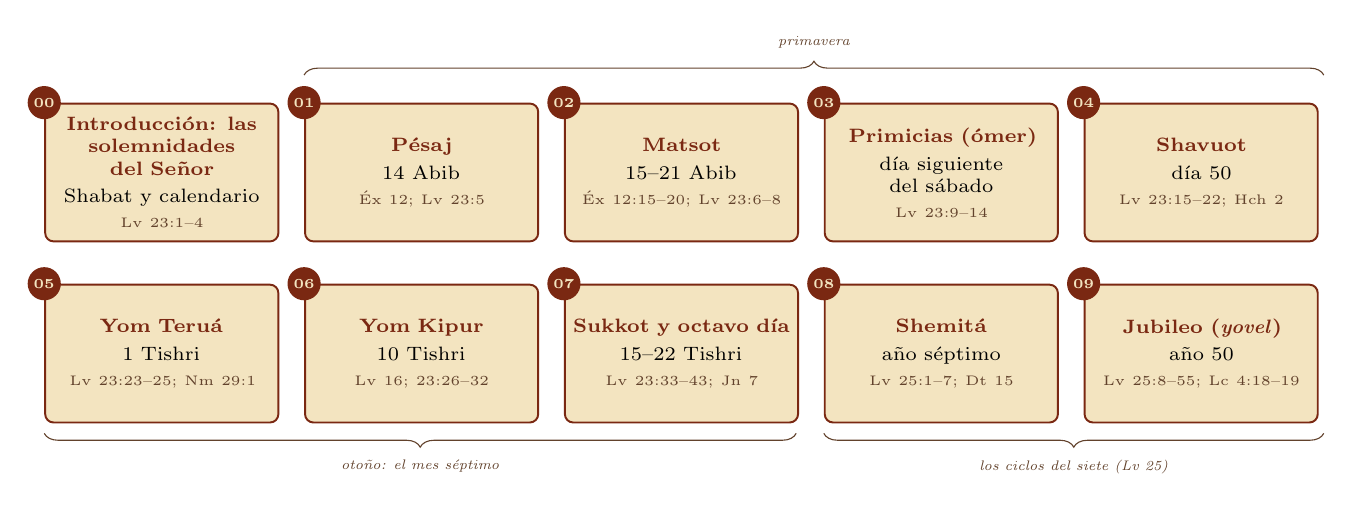
\begin{tikzpicture}[font=\scriptsize]
 \foreach \n/\t/\f/\r/\x/\y in {00/{Introducción: las solemnidades del \SENOR}/{Shabat y calendario}/{Lv 23:1--4}/0/0, 01/{Pésaj}/{14 Abib}/{Éx 12; Lv 23:5}/3.3/0, 02/{Matsot}/{15--21 Abib}/{Éx 12:15--20; Lv 23:6--8}/6.6/0, 03/{Primicias (ómer)}/{día siguiente del sábado}/{Lv 23:9--14}/9.9/0, 04/{Shavuot}/{día 50}/{Lv 23:15--22; Hch 2}/13.2/0, 05/{Yom Teruá}/{1 Tishri}/{Lv 23:23--25; Nm 29:1}/0/-2.3, 06/{Yom Kipur}/{10 Tishri}/{Lv 16; 23:26--32}/3.3/-2.3, 07/{Sukkot y octavo día}/{15--22 Tishri}/{Lv 23:33--43; Jn 7}/6.6/-2.3, 08/{Shemitá}/{año séptimo}/{Lv 25:1--7; Dt 15}/9.9/-2.3, 09/{Jubileo (\emph{yovel})}/{año 50}/{Lv 25:8--55; Lc 4:18--19}/13.2/-2.3}{
   \node[draw=tierraroja,line width=0.7pt,fill=papiro,rounded corners=3pt,text width=2.75cm,minimum height=1.75cm,align=center,inner sep=3pt,anchor=north west] (m\n) at (\x,\y) {\textbf{\textcolor{tierraroja}{\t}}\\[2pt] \f\\[1pt] {\tiny\color{sepia}\r}};
   \node[circle,fill=tierraroja,text=papiro,font=\tiny\bfseries,inner sep=1.4pt] at (m\n.north west) {\n};}
 \draw[decorate,decoration={brace,amplitude=5pt},sepia] (3.3,0.35) -- (16.25,0.35) node[midway,above=6pt,font=\tiny\itshape,text=sepia] {primavera};
 \draw[decorate,decoration={brace,amplitude=5pt,mirror},sepia] (0,-4.2) -- (9.55,-4.2) node[midway,below=6pt,font=\tiny\itshape,text=sepia] {otoño: el mes séptimo};
 \draw[decorate,decoration={brace,amplitude=5pt,mirror},sepia] (9.9,-4.2) -- (16.25,-4.2) node[midway,below=6pt,font=\tiny\itshape,text=sepia] {los ciclos del siete (Lv 25)};
\end{tikzpicture}\par
{\footnotesize\color{sepia}\textit{Figura 10.} Los diez estudios de la serie \emph{Festividades santas}. \textit{Nota.} Elaboración propia.}
\end{center}

Cada estudio sigue el mismo método: el texto en sus fuentes, la historia, la filología, la crítica textual, la forma literaria, la lectura de la serie con sus precisiones, el Nuevo Testamento, la tradición judía y la discusión. El orden reproduce el del año: comenzamos donde comenzó la libertad de Israel, en el mes de Abib, y terminamos en el año en que cada uno vuelve a su posesión.

%===================================================================
\section*{Glosario}\markboth{Glosario}{}
\begin{description}\setlength{\itemsep}{2pt}
\item[Abib] (\heb{אָבִיב}). ``Espiga verde''. Nombre antiguo del primer mes (Éx 13:4; Dt 16:1), llamado Nisán después del exilio.
\item[Atséret] (\heb{עֲצֶרֶת}). ``Asamblea de clausura''. Nombre del octavo día de Sukkot (Lv 23:36) y, en la tradición, de Shavuot.
\item[Calendario lunisolar] Sistema de meses lunares ajustados al año solar mediante un mes intercalar (Adar II o Veadar).
\item[Jag] (\heb{חַג}). Fiesta de peregrinación: Matsot, Shavuot y Sukkot (Dt 16:16). Cognado del árabe \emph{ḥajj}.
\item[Jódesh] (\heb{חֹדֶשׁ}). ``Luna nueva'' y ``mes''. \emph{Rosh jódesh}: el comienzo del mes (Nm 10:10; 28:11).
\item[Jukat olam] (\heb{חֻקַּת עוֹלָם}). ``Estatuto perpetuo'', fórmula de permanencia por las generaciones (Lv 23:14, 21, 31, 41).
\item[Melejet avodá] (\heb{מְלֶאכֶת עֲבֹדָה}). ``Trabajo de siervos'', labor ordinaria prohibida en los días santos anuales; distinto de \emph{kol melajá}, ``todo trabajo'', prohibido en Shabat y Kipur.
\item[Mikrá kódesh] (\heb{מִקְרָא קֹדֶשׁ}). ``Santa convocación''; de \emph{k-r-'}, ``llamar, leer''. LXX \grc{κλητὴ ἁγία}.
\item[Moed, moadim] (\heb{מוֹעֵד}, \heb{מוֹעֲדִים}). ``Cita, tiempo señalado, lugar de encuentro''; de \emph{y-'-d}. \emph{Moadé YHWH}: ``las fiestas solemnes del \SENOR'' (Lv 23:2).
\item[Óhel moed] (\heb{אֹהֶל מוֹעֵד}). ``Tabernáculo de reunión'', donde Dios ``se reúne'' con Israel (Éx 29:42).
\item[Sabbatismós] (\grc{σαββατισμός}). ``Reposo sabático'' que ``queda para el pueblo de Dios'' (He 4:9).
\item[Shabat] (\heb{שַׁבָּת}). ``Cese, reposo''; el séptimo día (Gn 2:2--3; Lv 23:3).
\item[Shabatón] (\heb{שַׁבָּתוֹן}). ``Reposo solemne''. \emph{Shabat shabatón}: Shabat, Kipur y año sabático.
\item[Shalosh regalim] (\heb{שָׁלֹשׁ רְגָלִים}). ``Tres veces'' (lit. ``tres pies''): las tres peregrinaciones (Éx 23:14).
\item[Shemitá] (\heb{שְׁמִטָּה}). ``Remisión''; el año séptimo de descanso de la tierra y de remisión de deudas (Dt 15:1--2; Lv 25:1--7).
\item[Tekufá] (\heb{תְּקוּפָה}). ``Vuelta'' del año (Éx 34:22); en la tradición, el punto solar que regula la intercalación.
\item[Yovel] (\heb{יוֹבֵל}). Jubileo, el año cincuenta, proclamado con trompeta el día de la expiación (Lv 25:8--10).
\item[Zikarón] (\heb{זִכָּרוֹן}). ``Memorial''; la Pascua (Éx 12:14), \emph{zijrón teruá} (Lv 23:24). LXX \grc{μνημόσυνον}.
\end{description}

%===================================================================
\section*{Referencias}\markboth{Referencias}{}
\refapa{Attridge, H.~W. (1989). \emph{The epistle to the Hebrews} (Hermeneia). Fortress Press.}
\refapa{Bacchiocchi, S. (1977). \emph{From Sabbath to Sunday: A historical investigation of the rise of Sunday observance in early Christianity}. Pontifical Gregorian University Press.}
\refapa{Bauer, W., Danker, F.~W., Arndt, W.~F., \& Gingrich, F.~W. (2000). \emph{A Greek-English lexicon of the New Testament and other early Christian literature} (3.ª ed.). University of Chicago Press.}
\refapa{Botterweck, G.~J., \& Ringgren, H. (Eds.). (1974--2006). \emph{Theological dictionary of the Old Testament} (15 vols.). Eerdmans.}
\refapa{Brown, F., Driver, S.~R., \& Briggs, C.~A. (1906). \emph{A Hebrew and English lexicon of the Old Testament}. Clarendon Press.}
\refapa{Carson, D.~A. (Ed.). (1982). \emph{From Sabbath to Lord's Day: A biblical, historical, and theological investigation}. Zondervan.}
\refapa{Chumney, E. (1994). \emph{The seven festivals of the Messiah}. Destiny Image.}
\refapa{Danby, H. (Trad.). (1933). \emph{The Mishnah}. Oxford University Press.}
\refapa{de Vaux, R. (1985). \emph{Instituciones del Antiguo Testamento} (4.ª ed.). Herder.}
\refapa{Dunn, J.~D.~G. (1998). \emph{The theology of Paul the apostle}. Eerdmans.}
\refapa{Elliger, K., \& Rudolph, W. (Eds.). (1997). \emph{Biblia Hebraica Stuttgartensia} (5.ª ed.). Deutsche Bibelgesellschaft.}
\refapa{Eusebio de Cesarea. (1926--1932). \emph{The ecclesiastical history} (K. Lake \& J.~E.~L. Oulton, Trads.; 2 vols.). Harvard University Press.}
\refapa{Fee, G.~D. (1987). \emph{The first epistle to the Corinthians} (NICNT). Eerdmans.}
\refapa{Filón de Alejandría. (1937). \emph{On the special laws} (F.~H. Colson, Trad.; Philo, Vol. 7). Harvard University Press.}
\refapa{García Martínez, F. (1992). \emph{Textos de Qumrán}. Trotta.}
\refapa{Hartley, J.~E. (1992). \emph{Leviticus} (WBC 4). Word Books.}
\refapa{Hays, R.~B. (1989). \emph{Echoes of Scripture in the letters of Paul}. Yale University Press.}
\refapa{Heschel, A.~J. (1951). \emph{The Sabbath: Its meaning for modern man}. Farrar, Straus and Young.}
\refapa{Josefo, F. (1997). \emph{Antigüedades judías} (J. Vara Donado, Trad.). Akal.}
\refapa{Keener, C.~S. (2003). \emph{The Gospel of John: A commentary} (2 vols.). Hendrickson.}
\refapa{Koehler, L., \& Baumgartner, W. (2001). \emph{The Hebrew and Aramaic lexicon of the Old Testament} (Ed. de estudio). Brill.}
\refapa{Lane, W.~L. (1991). \emph{Hebrews} (WBC 47A--B). Word Books.}
\refapa{Levine, B.~A. (1989). \emph{Leviticus} (JPS Torah Commentary). Jewish Publication Society.}
\refapa{Martin, T.~W. (1996). Pagan and Judeo-Christian time-keeping schemes in Galatians 4.10 and Colossians 2.16. \emph{New Testament Studies}, \emph{42}(1), 105--119.}
\refapa{Milgrom, J. (2001). \emph{Leviticus 23--27} (Anchor Bible 3B). Doubleday.}
\refapa{Moo, D.~J. (1996). \emph{The epistle to the Romans} (NICNT). Eerdmans.}
\refapa{Nestle, E., \& Aland, K. (Eds.). (2012). \emph{Novum Testamentum Graece} (28.ª ed.). Deutsche Bibelgesellschaft.}
\refapa{Propp, W.~H.~C. (1999). \emph{Exodus 1--18} (Anchor Bible 2). Doubleday.}
\refapa{Rahlfs, A., \& Hanhart, R. (Eds.). (2006). \emph{Septuaginta} (ed. rev.). Deutsche Bibelgesellschaft.}
\refapa{Sarna, N.~M. (1991). \emph{Exodus} (JPS Torah Commentary). Jewish Publication Society.}
\refapa{Sefaria. (s.~f.). \emph{Sefaria: A living library of Jewish texts}. https://www.sefaria.org}
\refapa{Sociedades Bíblicas en América Latina. (1960). \emph{Santa Biblia: Reina-Valera 1960}.}
\refapa{Tigay, J.~H. (1996). \emph{Deuteronomy} (JPS Torah Commentary). Jewish Publication Society.}
\refapa{VanderKam, J.~C. (1998). \emph{Calendars in the Dead Sea Scrolls: Measuring time}. Routledge.}
\refapa{Wenham, G.~J. (1979). \emph{The book of Leviticus} (NICOT). Eerdmans.}
\refapa{Wenham, G.~J. (1987). \emph{Genesis 1--15} (WBC 1). Word Books.}
\refapa{Wright, N.~T. (2013). \emph{Paul and the faithfulness of God}. Fortress Press.}

\end{document}
